% !TEX root = ../Rulebook.tex
\label{sec:Tests}

\section{General}

\subsection{Common Rules}
\label{ssec: Common Rules}


Unless stated other, the following rules apply to all test types:

\begin{itemize}
\item The order in which the teams have to perform will be determined by a draw from the OC.
\item The prep phase has a time limit of 3 minutes.
\item Teams must not hardcode information gained from runs of previous teams. This is considered as cheating.
\item A single robot is used.
\item The robot must not leave the arena.
\item Robots are allowed to carry three objects max. If more than 3 objects are above the robot's footprint, the same rule as for a major collision applies (run stopped or optional restart, stop after 2nd time). 
\item The robot has to start and end at the respective arena location (START, FINISH).
\item The robot will get the task specification from the AC or an official bagfile.
\item Reaching each active Service Area successfully is rewarded once with points defined in table \ref{fig:test_scoring}.
\item Service Areas count as succesfully reached as defined in section \ref{sec:ArenaDesign}.
\item Manipulation tasks count as successful as defined in \ref{ssec:GraspingObjects} and \ref{ssec:PlacingObjects}.
\item The score for each test will be calculated as defined in \ref{sec:ScoringAndRanking}.
\item Exact test specifications are displayed in table \ref{fig:test_specifications_instance}.
\end{itemize}


%\end{itemize}



%The actual competition contains of a set of so-called tests. 
%A test is specified in terms of it's purpose and focus, environment features and eventually manipulation objects involved. Further, a concrete specification of the task is given and the rules to be obeyed. 

%Each test has different variability dimensions. That is, which objects to be manipulated, how many locations to visit, from which height to grasp etc. The test instances for \YEAR are defined based on the general test description and can be seen in Section~\ref{sec:ScoringAndRanking}.




%Every test has some navigation to a service area involved in it. Successful navigation will be awarded in every test according to Table \ref{tab:InstancePoints}. A navigation to a service area is successful when the robot reached the service area as defined in section \ref{ssec:Navigating}. The rewarded points for navigation to a servie area will be only awarded once per service area.

\subsection{Grasping Objects} \label{ssec:GraspingObjects}

\textbf{General}

An Object counts as successfully grasped if the robot picks the correct Object type from the correct Service Area and carries it out of the Manipulation Zone, which is treated with imaginary boundaries of infinite height. 
The object must be above the robot's footprint for a successful grasp.

A robot is allowed to lift other Objects, as long as the Objects are not moved out of the Manipulation Zone with their complete form. 
This enables a robot to pick and inspect all Objects on the workstation with its camera from multiple angles. 
Removing an incorrect Object from the Manipulation zone is treated as an \texttt{Incorrect Object Manipulation}.

An \textbf{Object Loss} occurs when the robot drops an Object to either the floor or from a height of $5\si{\centi\meter}$ above the Service Area. If any Object (starts rolling and) falls off the edge of a Service Area after it has been touched by the robot, it is also considered as an \texttt{Object Loss}. 

The grasping process starts once the Manipulator enters the Manipulation Zone und ends when it leaves the Manipulation Zone.
If the robot collides with an Object, Decoy or Container inside the Manipulation Zone during the grasping process it is considered as a \texttt{Manipulation Deduction}.

To ensure objects are accessible on arbitrary surfaces, they must sink in no more than $\frac{1}{3}$ of their total height when placed on the surface. This means at least $\frac{2}{3}$  of the object's height must remain reachable from above without any obstructions by the arbitrary surface.


\textbf{Rotating Table}

It is explicitly NOT allowed to stop the table (e.g. by pushing the gripper into the table surface).

It is also explicitly NOT allowed to position the gripper in a way that blocks the objects 
unless it is during the grasping process of a target object and does not affect the table rotation or other objects.

A breach of one or both of these rules causes that no points are rewarded if the Object is successfully picked.

\subsection{Placing Objects} \label{ssec:PlacingObjects}

\textbf{General}

An Object counts as successfully placed if the robot places the correct Object type inside of the Manipulation Zone of the correct Service Area. The orientation of the object may be chosen freely by the robot, but the Object's footprint must lie completely inside of the Manipulation Zone.
Neither the placed object nor the robot are allowed to touch other Objects or Containers on the Service Area.
Breaches of these rules result in a \texttt{Manipulation Deduction}, which will only be applied once, independent of the actual amount of breaches, but for each grasping or placing.

If a placed Object either has an incorrect type or if it has been placed on the wrong Service Area, 
the placement is considered as an \texttt{Incorrect Object Manipulation}. 
Objects dropped from a height of $5\si{\centi\meter}$ or more above the Service Area are not counted as successfully placed but are rather treated as an \texttt{Object Loss}. This requires robots to carefully handle Objects as some might be damaged otherwise.


\textbf{Shelf}

Objects must be placed on the upper part of the Shelf.
The Manipulation Zone also applies for the tilted surface, but is extended until the edge of the Shelf to allow for Objects to slide down after a successful placement. Objects sliding onto other previously placed Objects cause a \texttt{Manipulation Deduction}.


\textbf{Precision Placement}

Objects must be placed onto the matching cavity tile with their complete form, which is then rewarded with a \texttt{Cavity Placement}.
If the object drops through the cavity and fully passes the cavity tile, the precision placement is considered as successful and is rewarded with an additional \texttt{Precision Placement}. 

It is allowed to perform form fitting strategies, such as wiggling the object after placement or using force sensors during manipulation,
as long as the cavity tile is not damaged during that process. A damaged cavity is treated as a \texttt{Incorrect Object Manipulation} and no points will be rewarded.

Objects placed on a mismatching cavity tile do not cause an \texttt{Incorrect Object Manipulation} penalty if they had to be precise placed in the first place. This relaxes the risk of performing this task as it reduces potential bad outcome from false cavity detections.
 

\textbf{Container Placement}

Container placements are considered as successful if an Object is placed inside of the container from a height less than $5\si{\centi\meter}$ above it's inside bottom. With container edges taller than $5\si{\centi\meter}$, robots must therefore "insert" their gripper fingers into the container during manipulation. Touching the container while placing the object is allowed, as long as the container is not moved substantially.
If the container moves more than $1\si{\centi\meter}$, is tilted or forcefully moved, a \texttt{Manipulation Deduction} penalty will be applied.

Placed Objects must touch the inside bottom of the container to count as successfully placed.
Figure \ref{fig:example_allenkeyOK} shows correct final object positions placement examples. 

\begin{figure}[h!]
	\begin{center}
		\subfloat{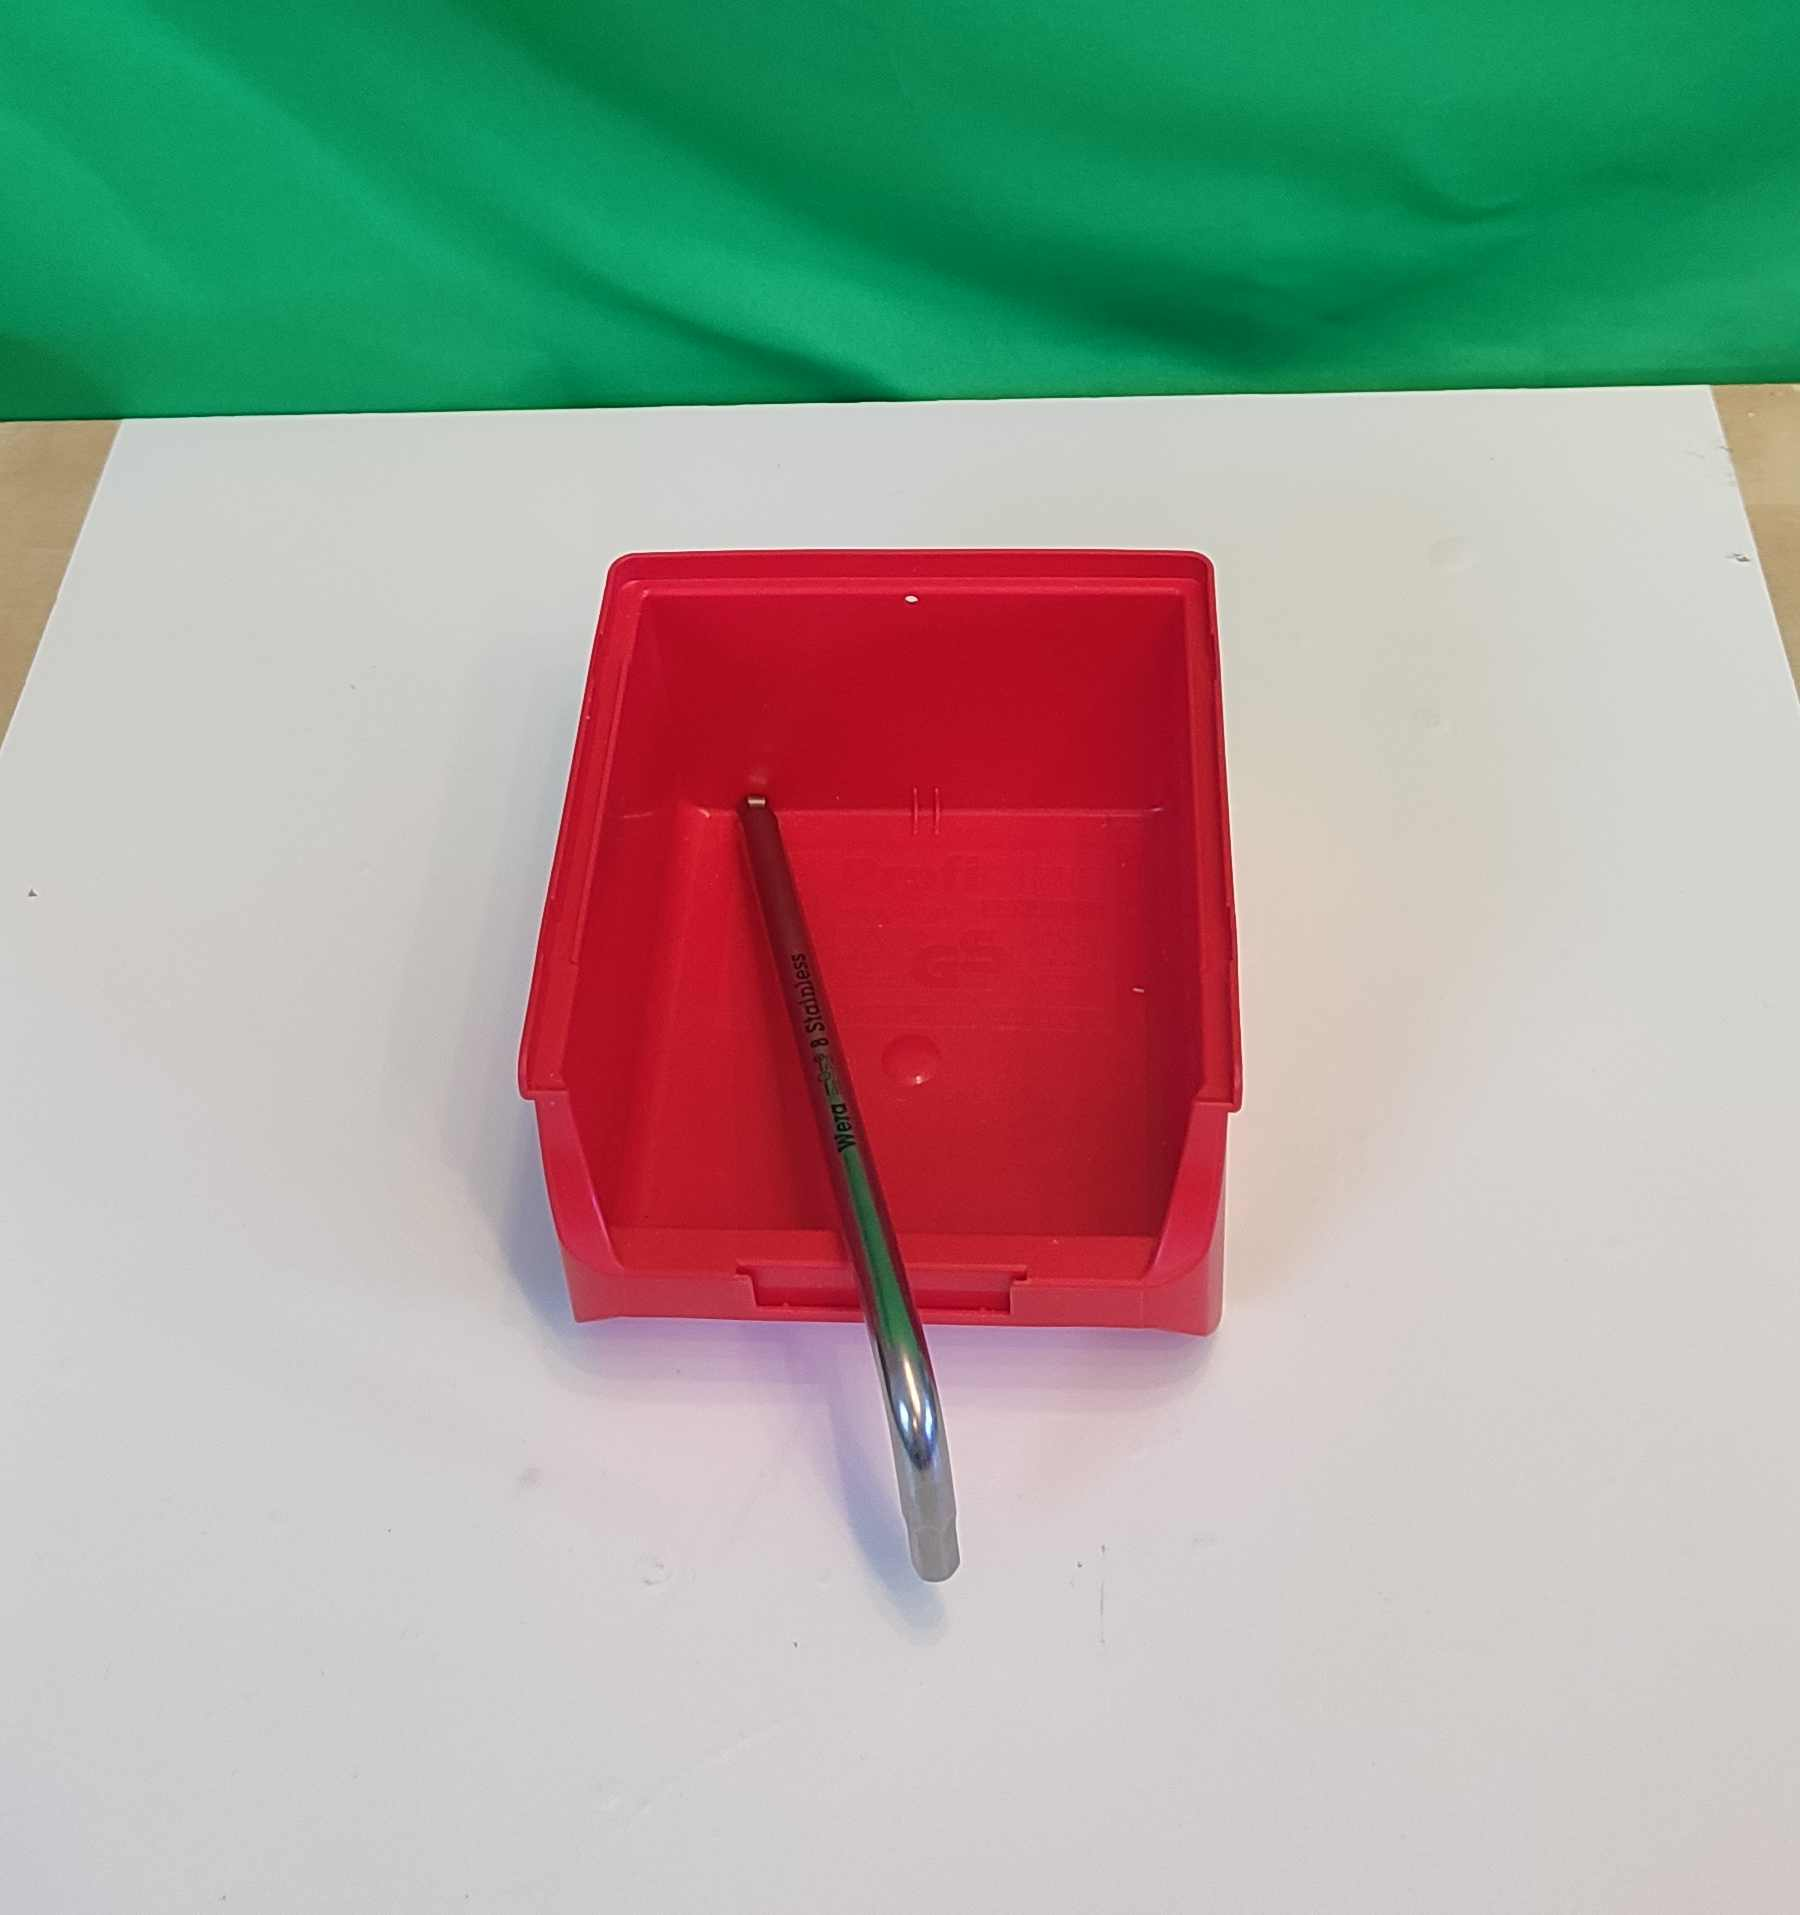
\includegraphics[width=0.24\textwidth,rotate=-0]{./images/placement_examples/allenkey_ok1.jpg}} \hfill
		\subfloat{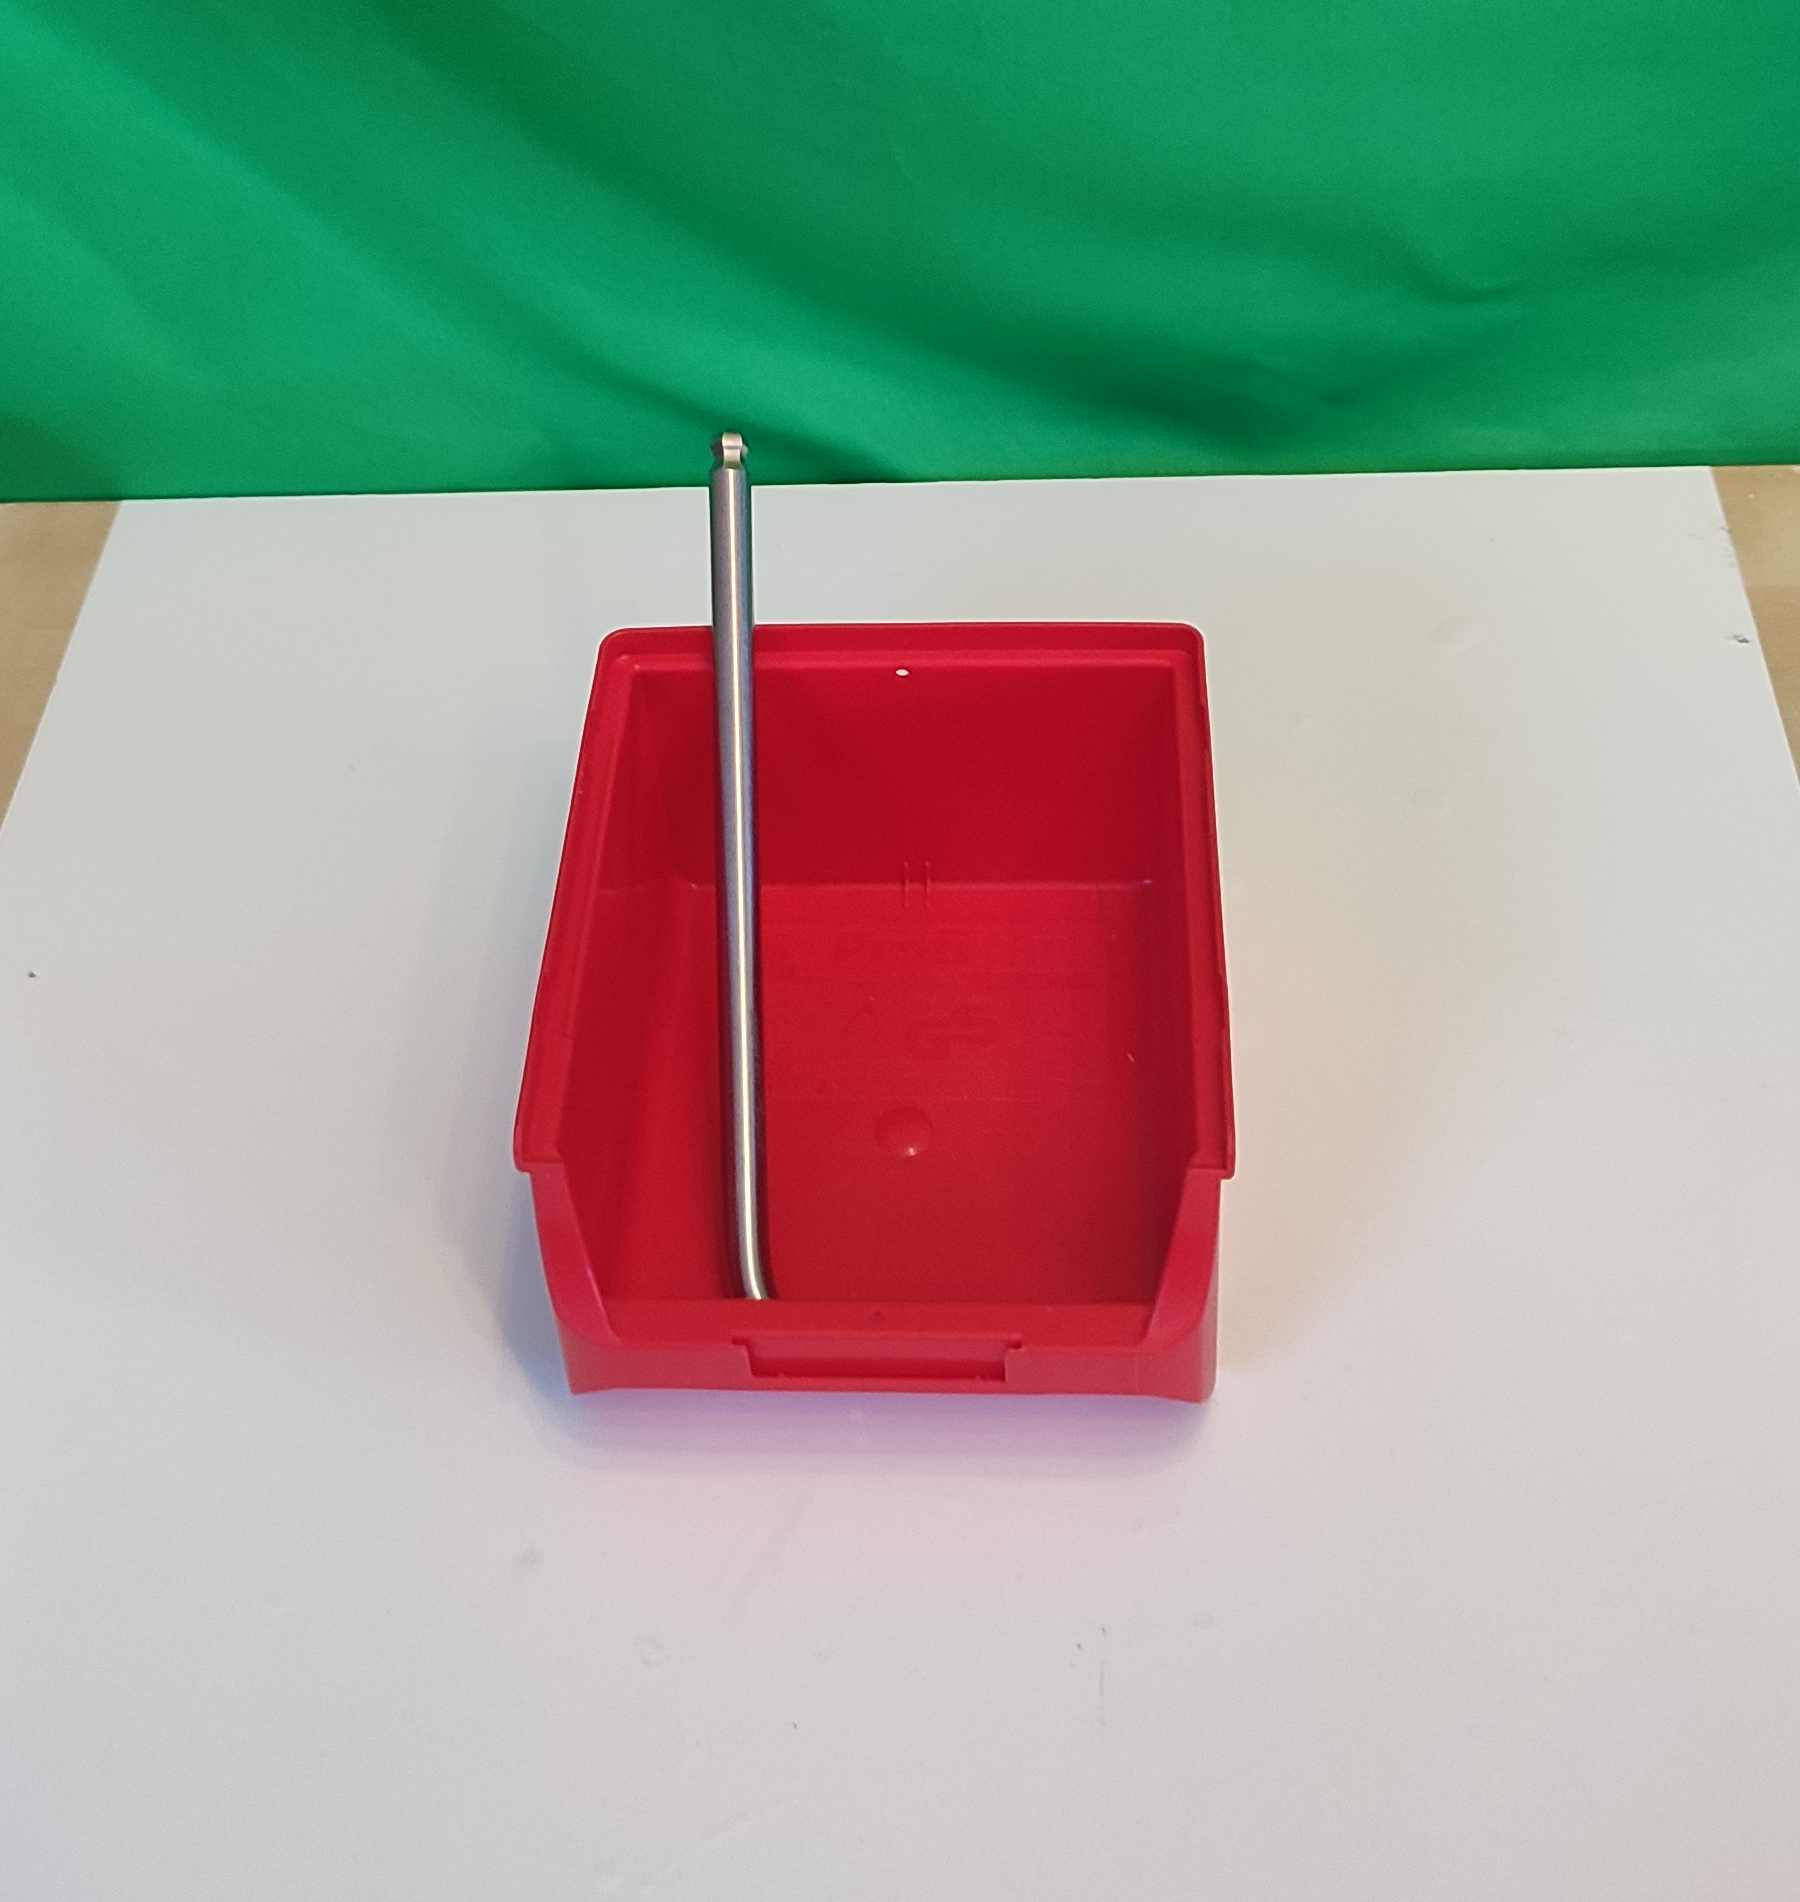
\includegraphics[width=0.24\textwidth,rotate=-0]{./images/placement_examples/allenkey_ok2.jpg}} \hfill
		\subfloat{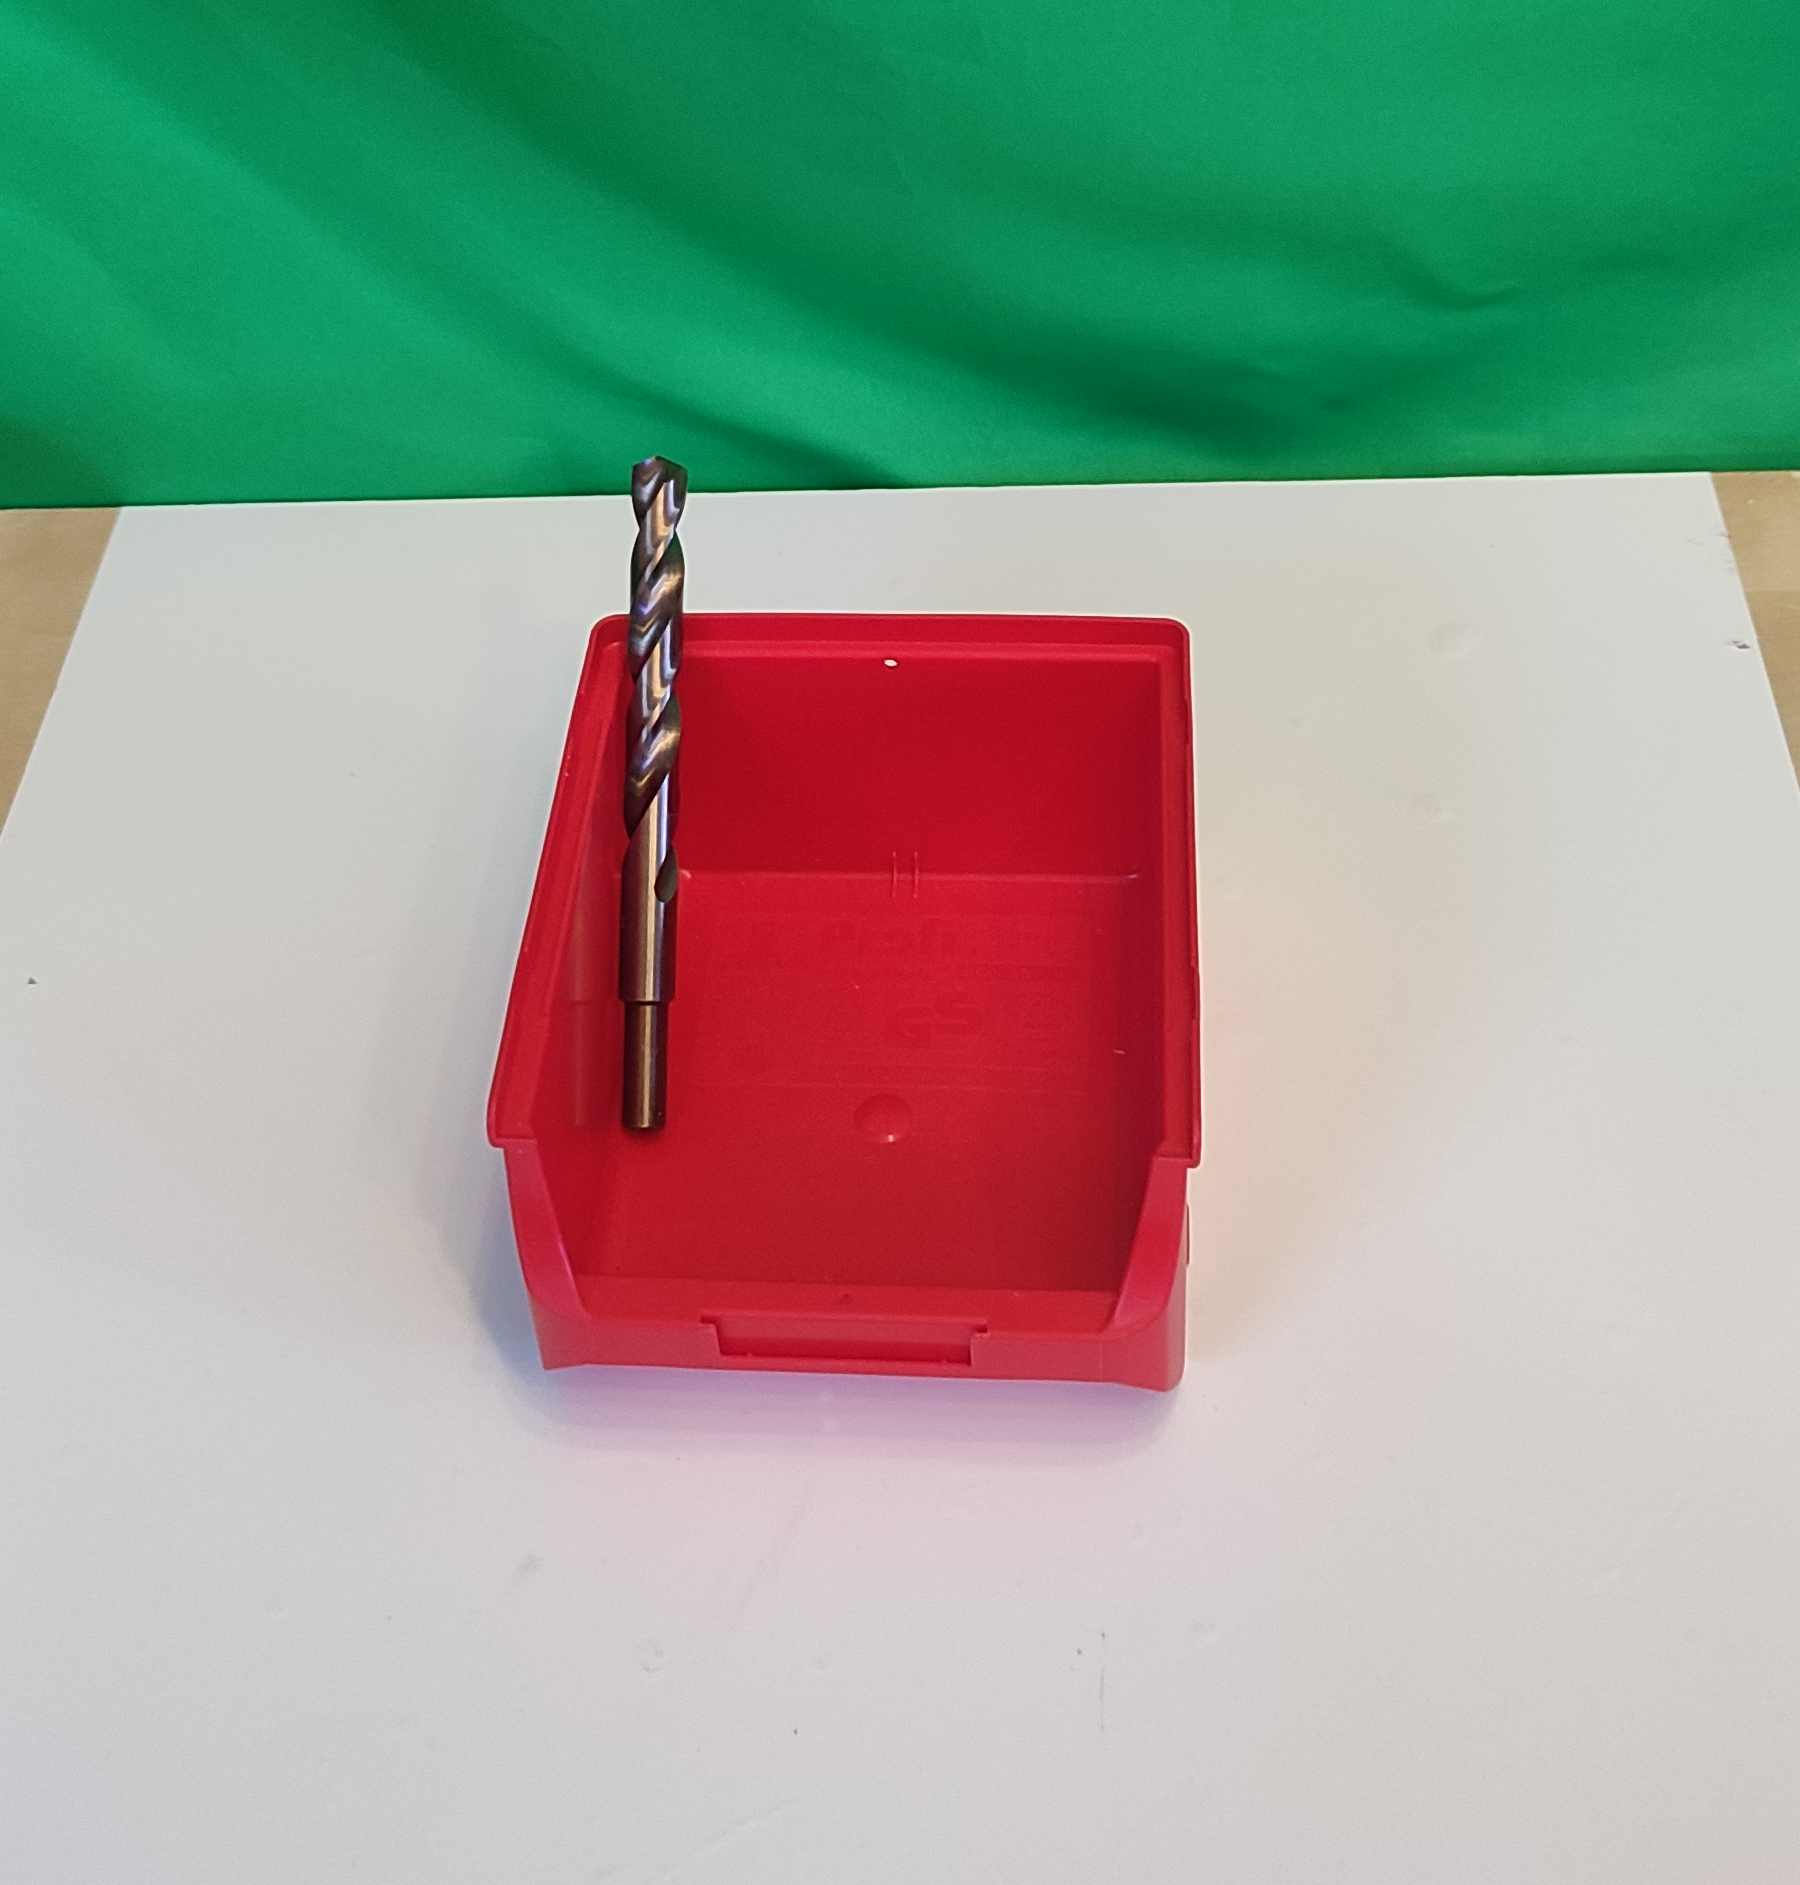
\includegraphics[width=0.24\textwidth,rotate=-0]{./images/placement_examples/drill_ok1.jpg}} \hfill
		\subfloat{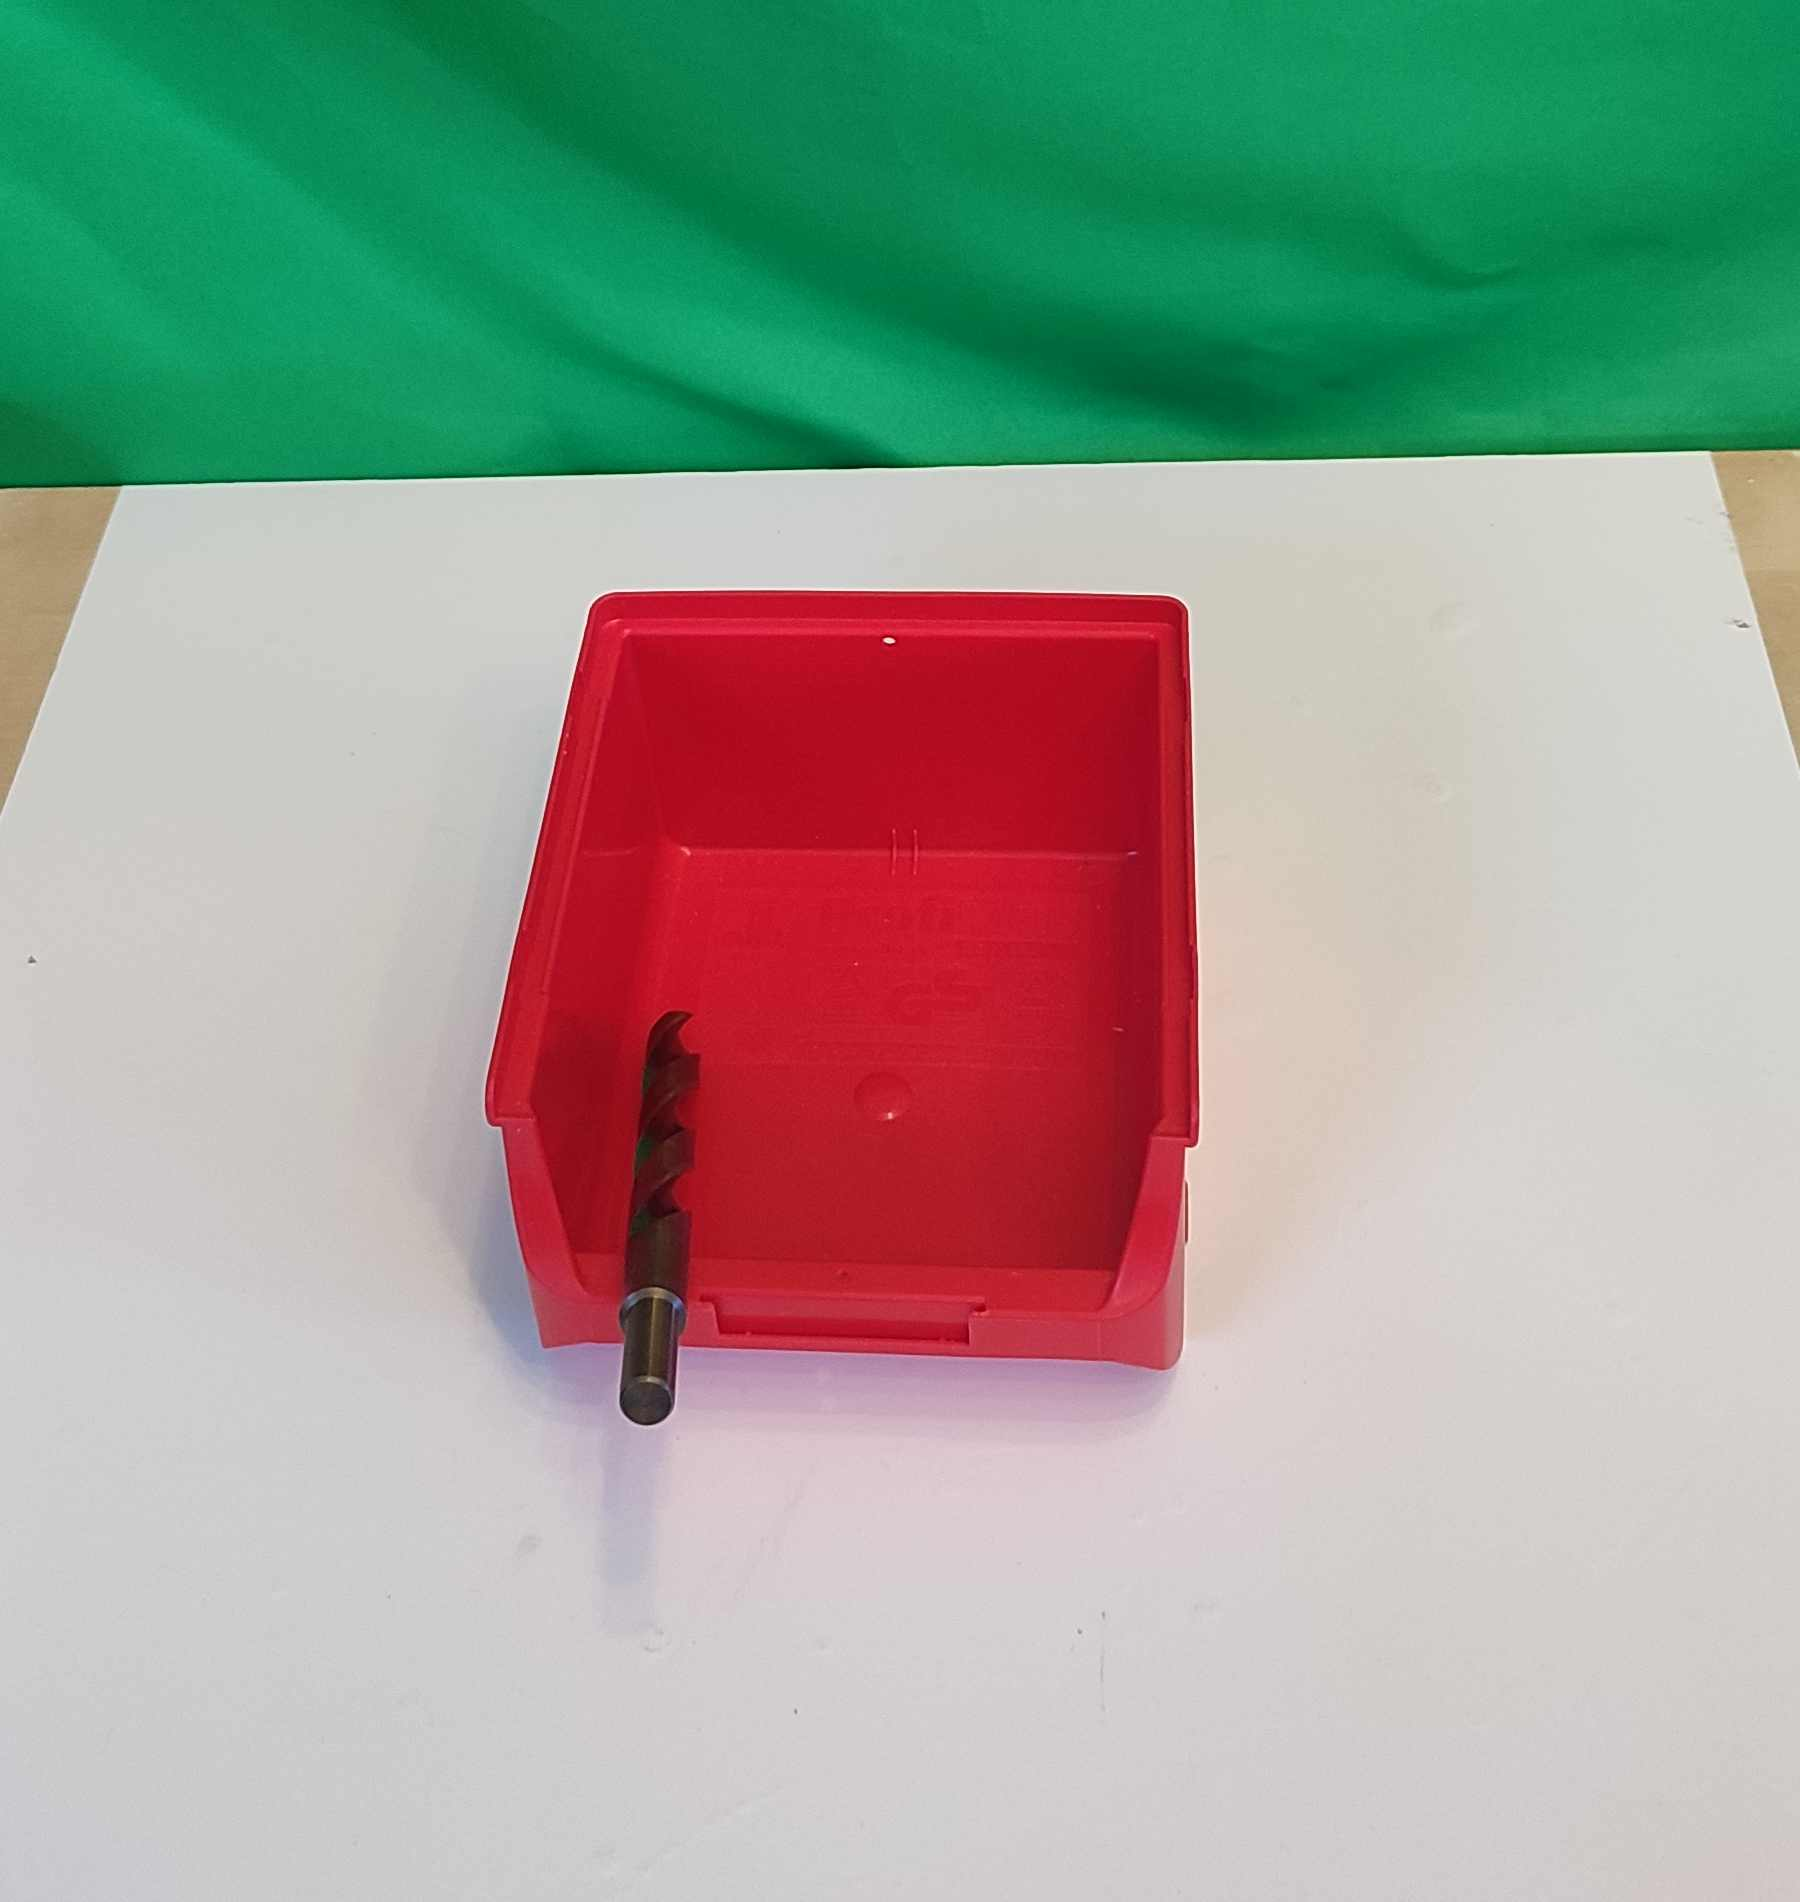
\includegraphics[width=0.24\textwidth,rotate=-0]{./images/placement_examples/drill_ok2.jpg}} \hfill
	\end{center}
	\caption{Examples of correct AllenKey and Drill in container placement.}
	\label{fig:example_allenkeyOK}
\end{figure}

Figure \ref{fig:example_allenkeyNOTOK} shows examples for incorrect placements, which cause a \texttt{Manipulation Deduction} and the bonus points for that container placement NOT being given. In this case, the placement is considered as a normal placement with all associated rules. 

\begin{figure}[h!]
	\begin{center}
		\subfloat{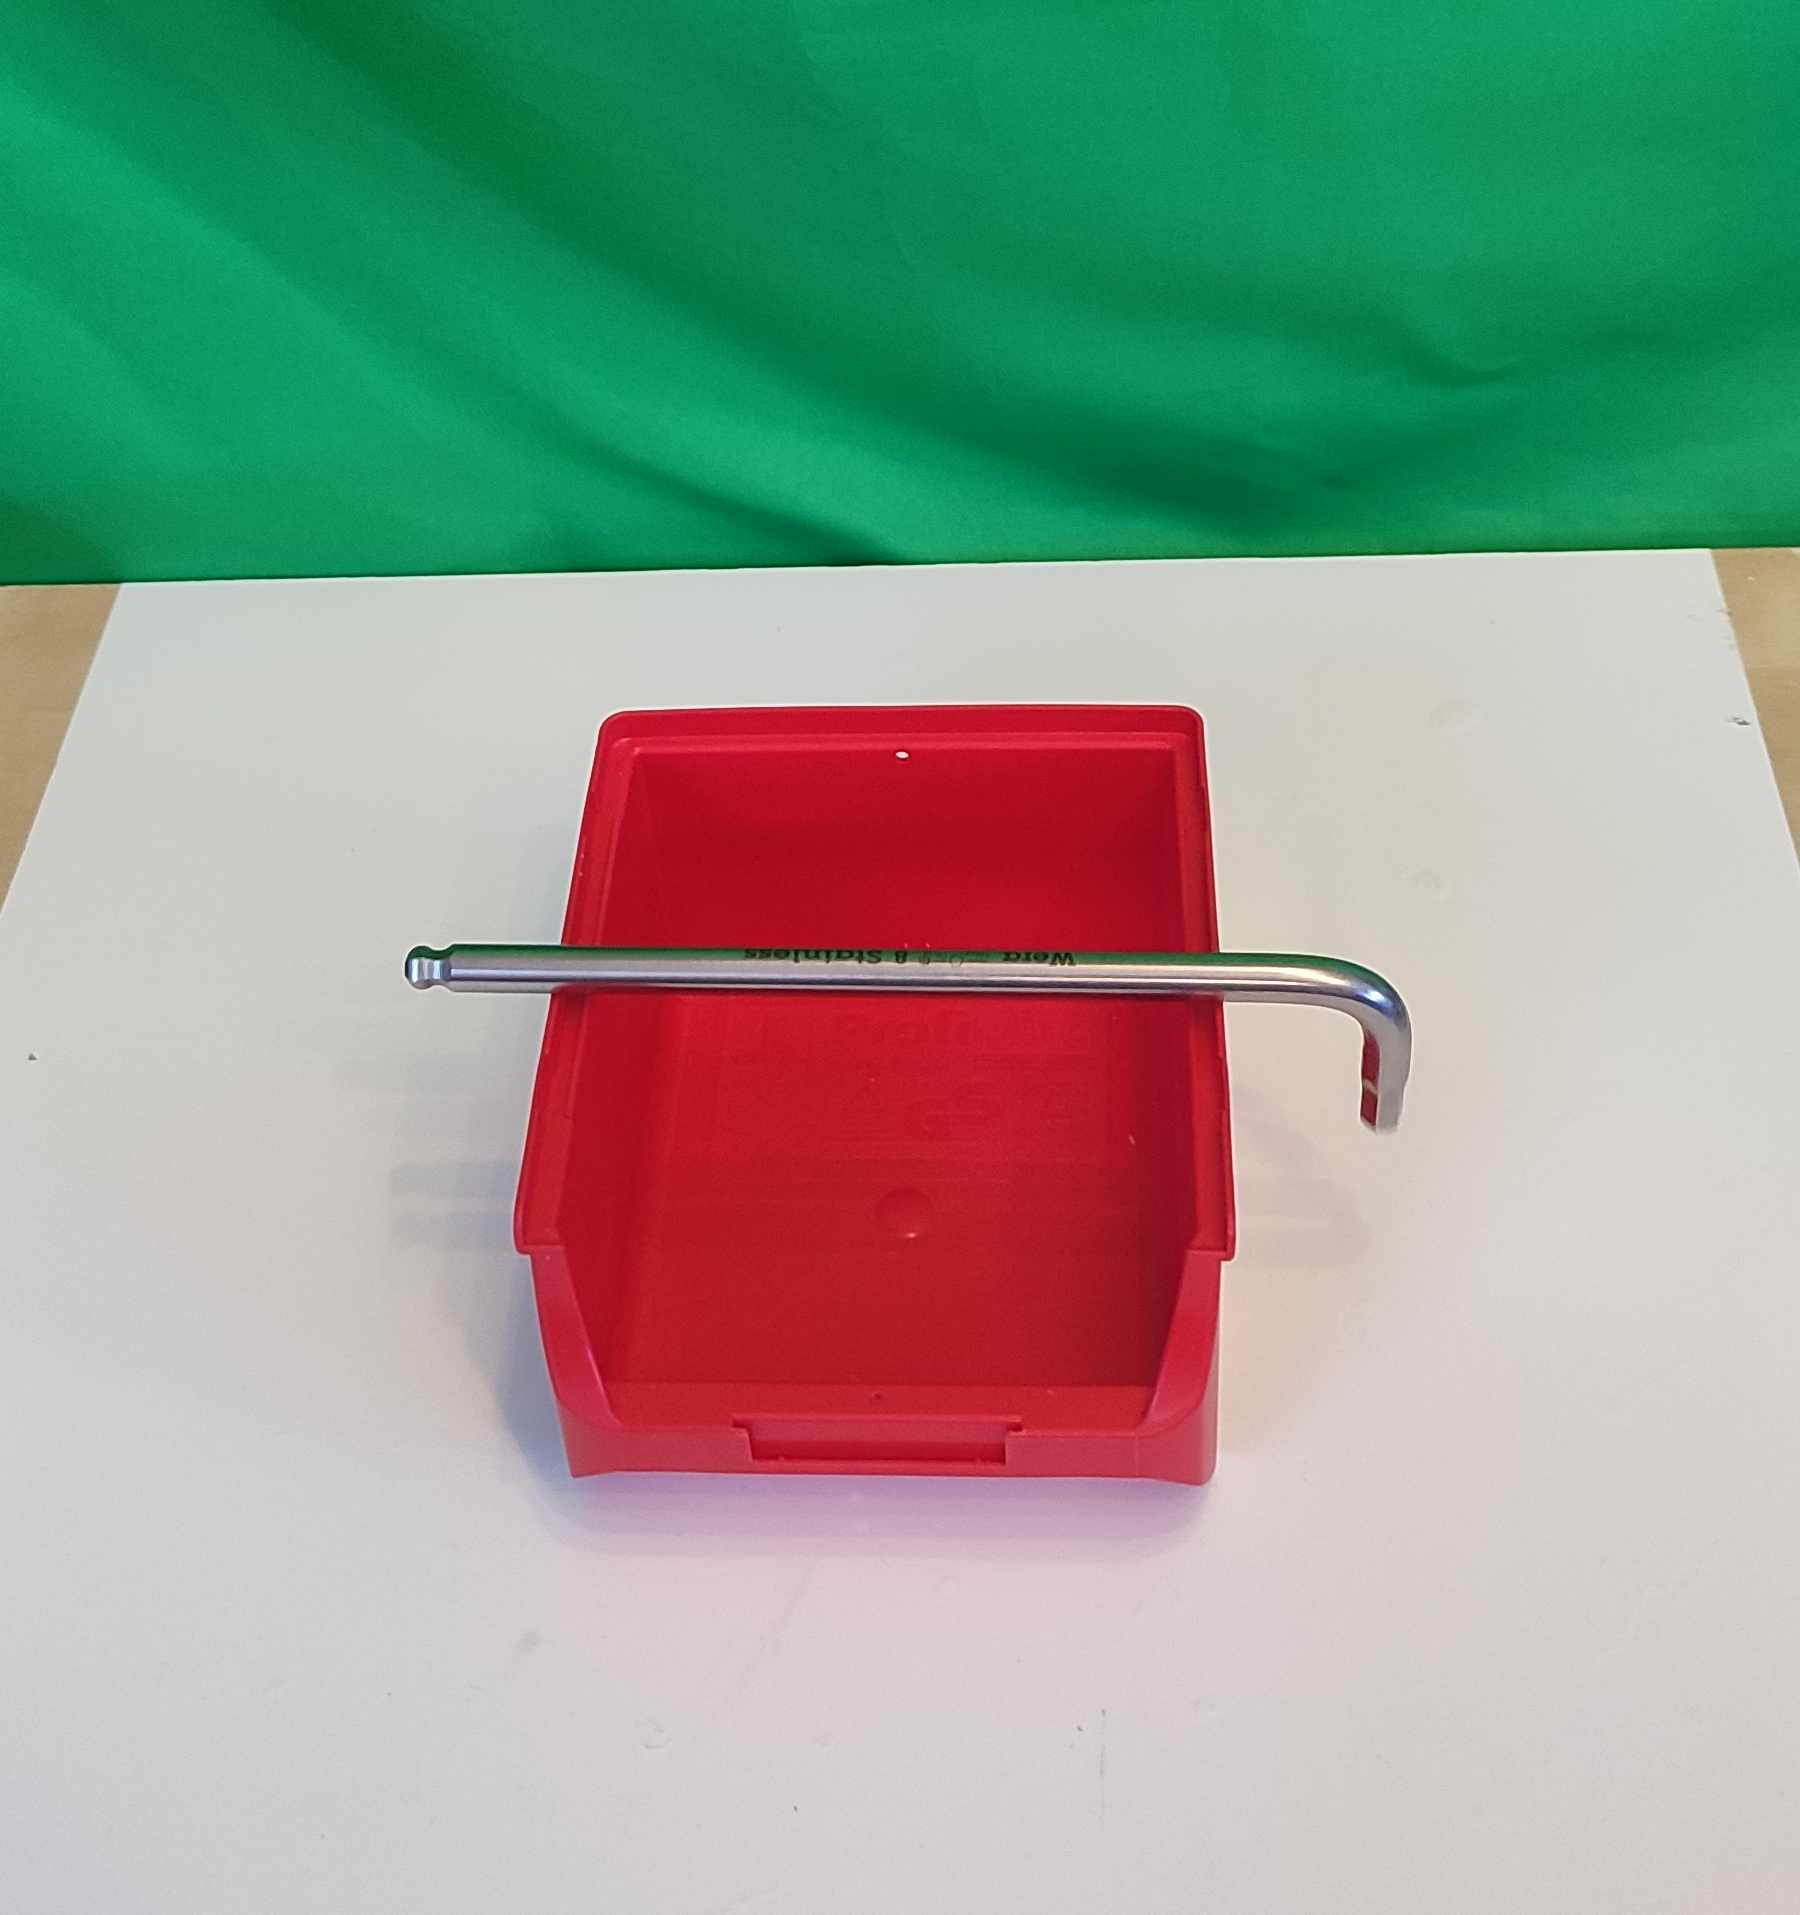
\includegraphics[width=0.24\textwidth,rotate=-0]{./images/placement_examples/allenkey_not_ok1.jpg}} \hfill
		\subfloat{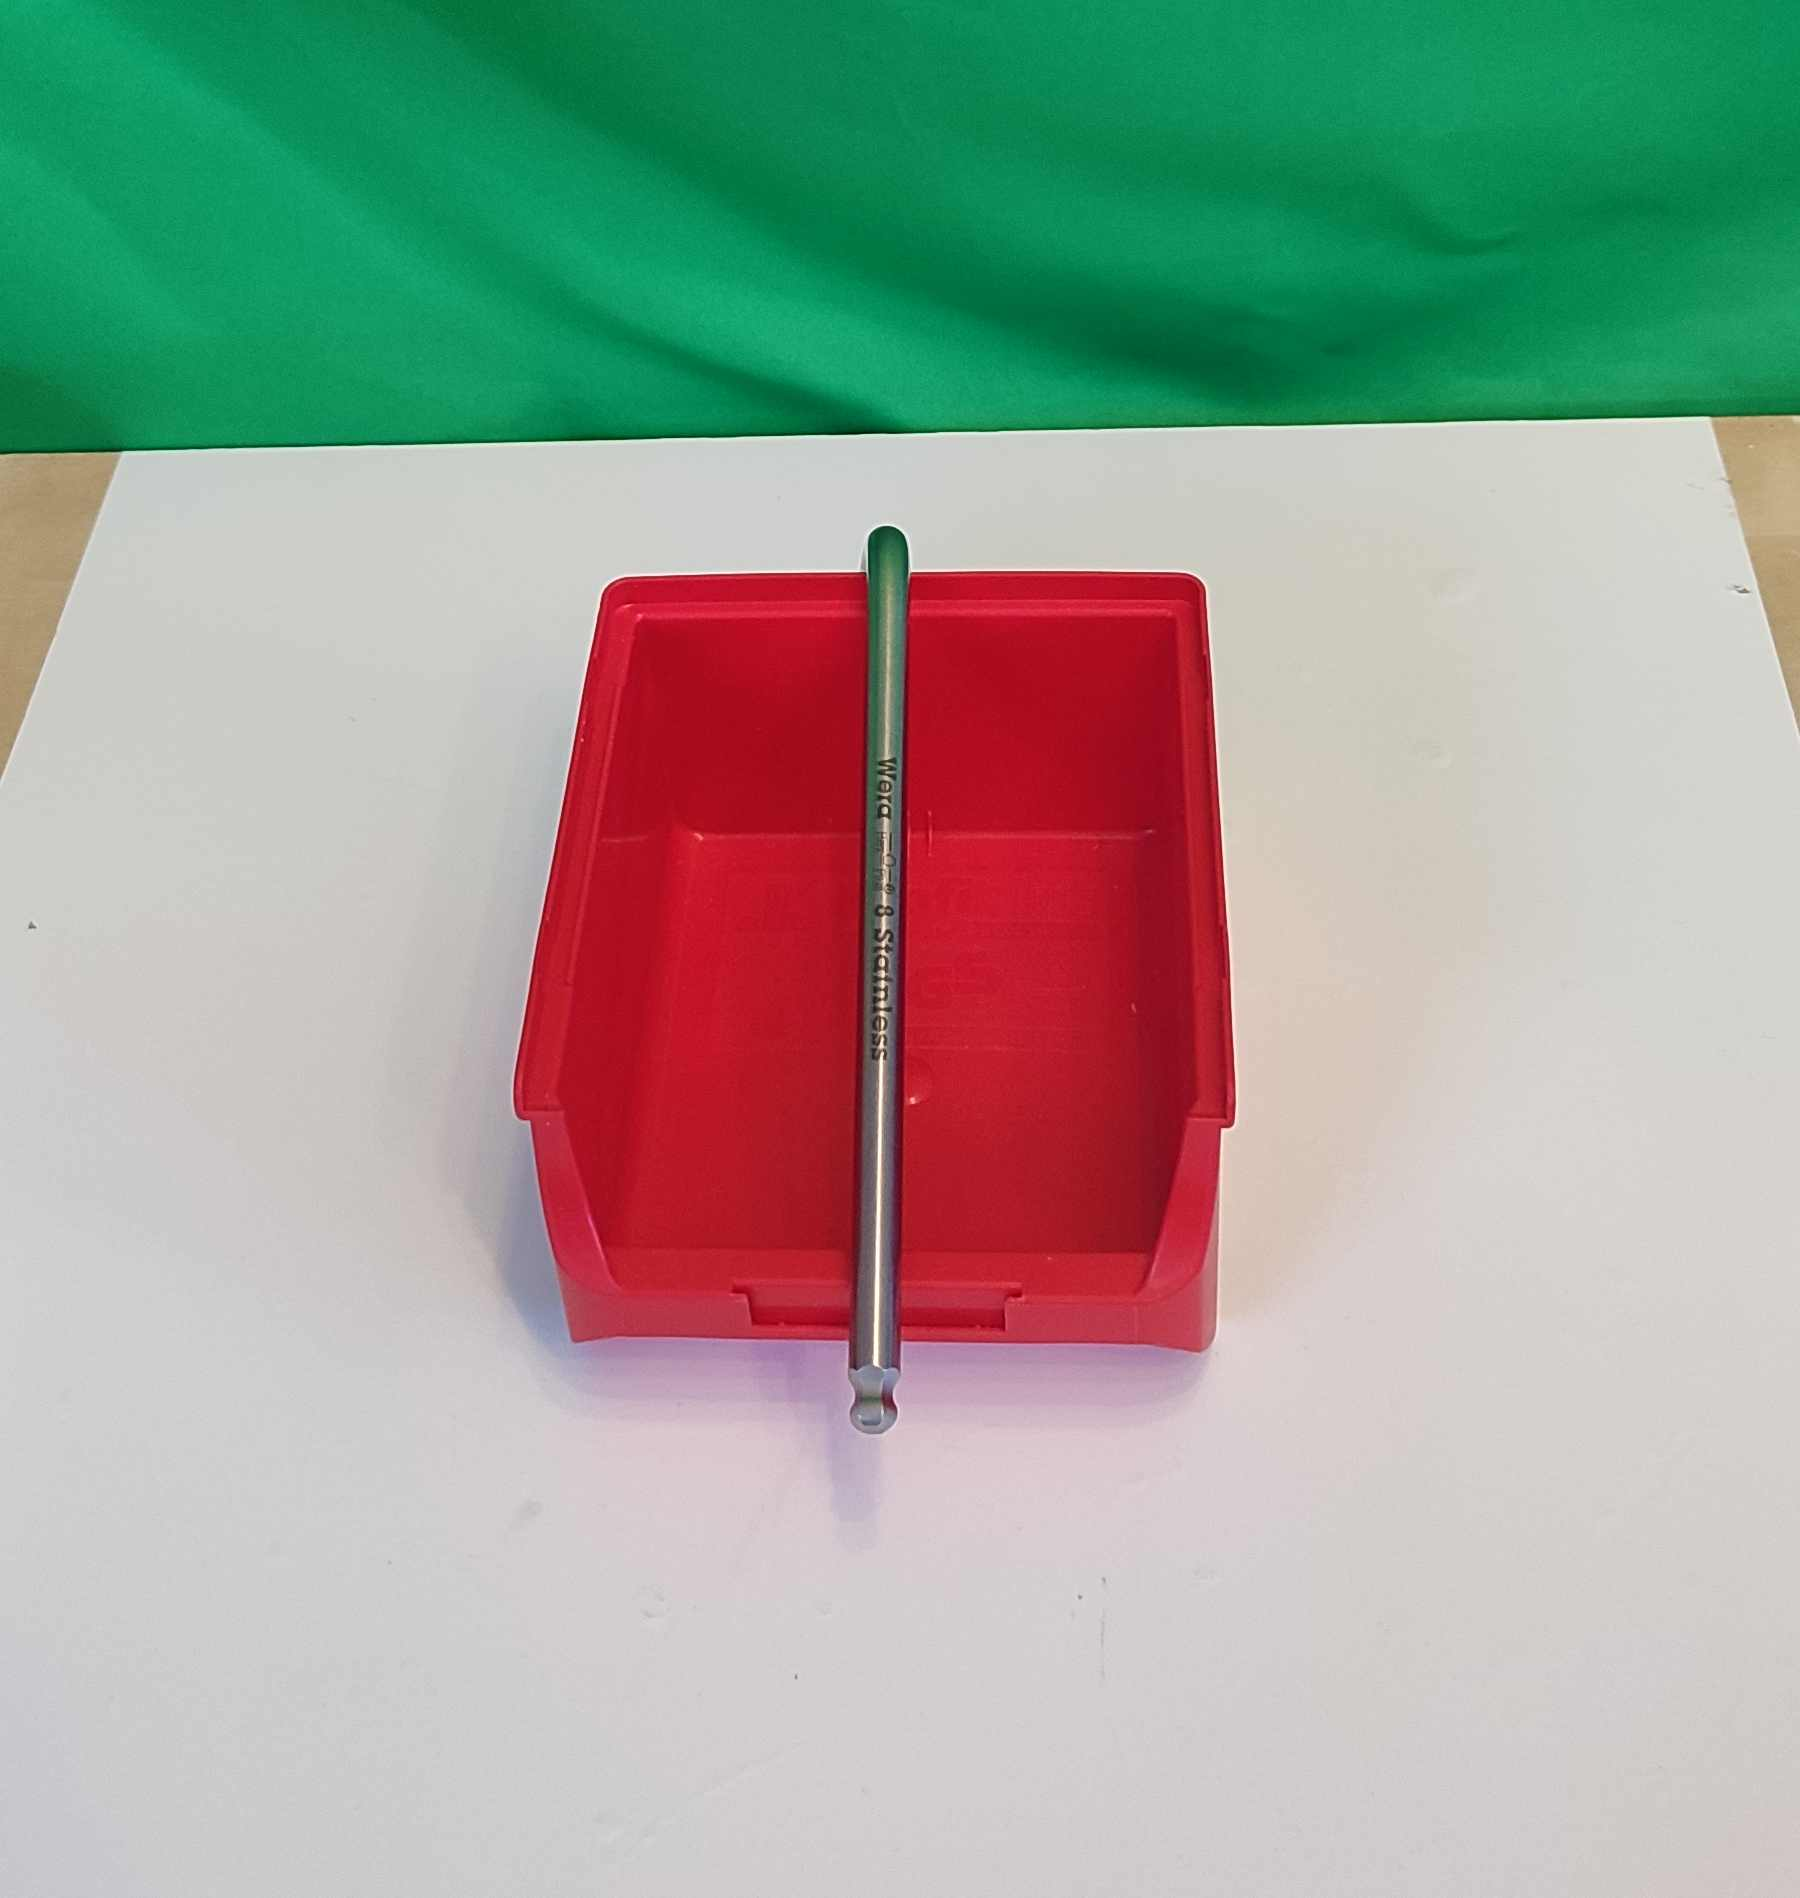
\includegraphics[width=0.24\textwidth,rotate=-0]{./images/placement_examples/allenkey_not_ok4.jpg}} \hfill
		\subfloat{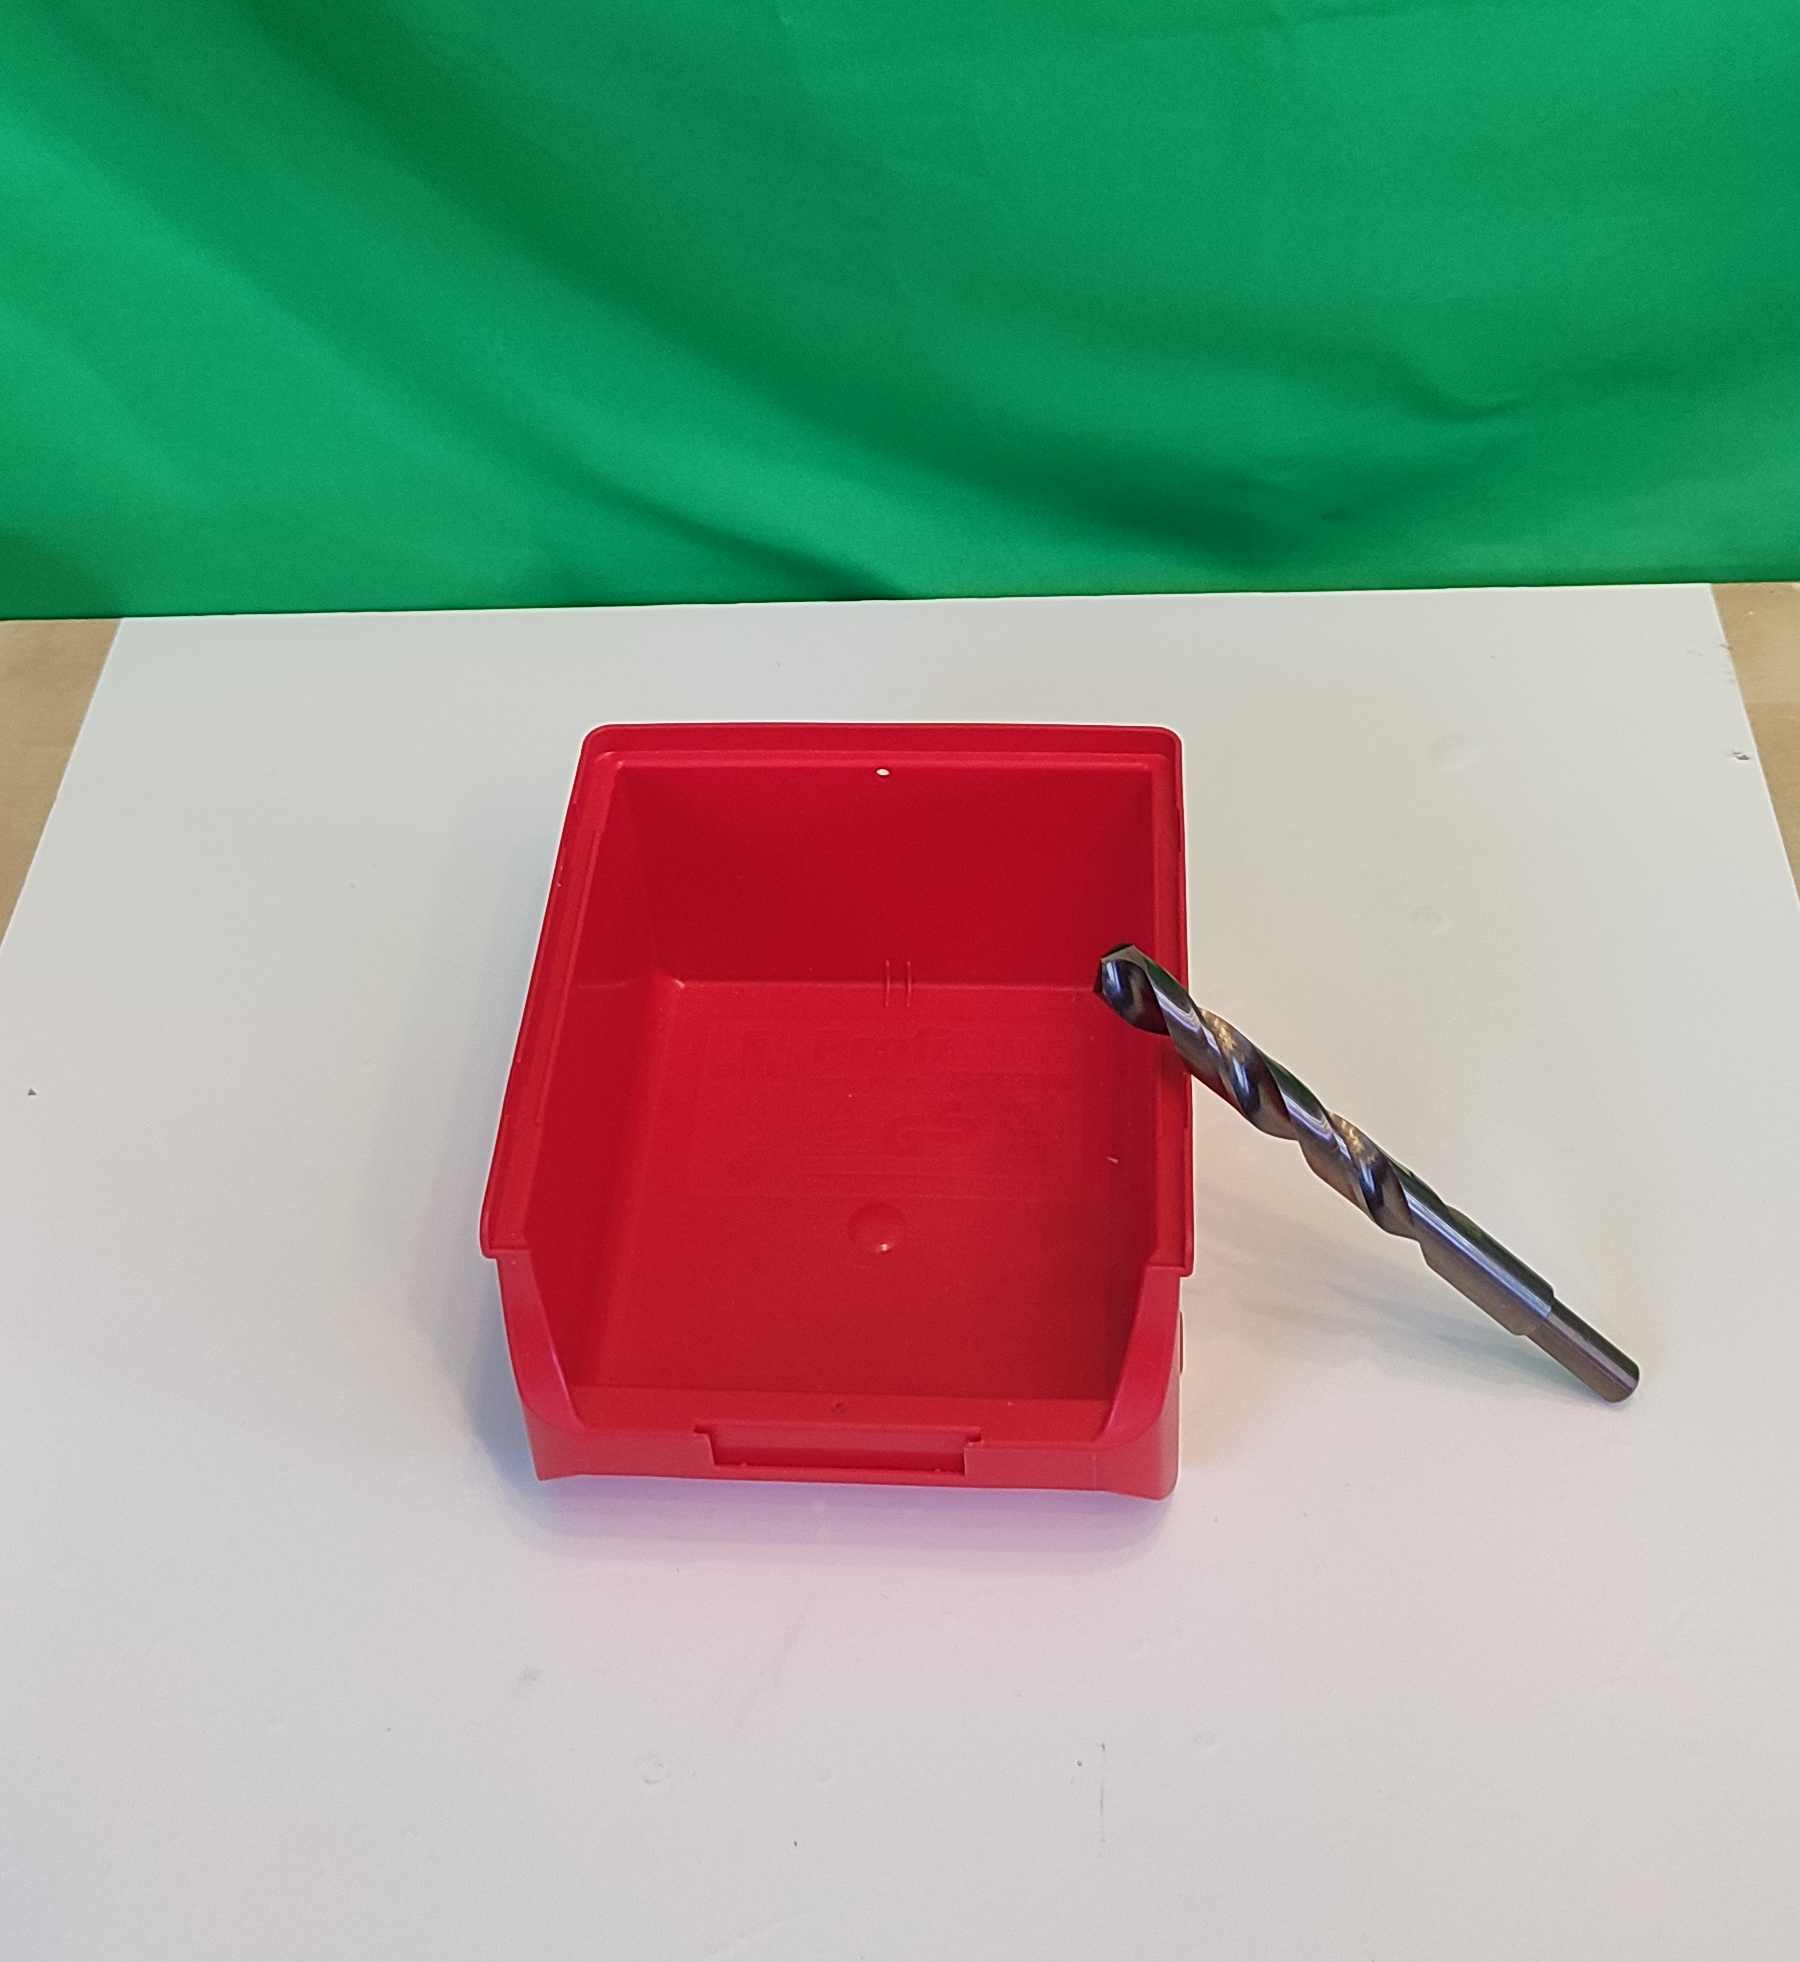
\includegraphics[width=0.24\textwidth,rotate=-0]{./images/placement_examples/drill_not_ok2.jpg}} \hfill
		\subfloat{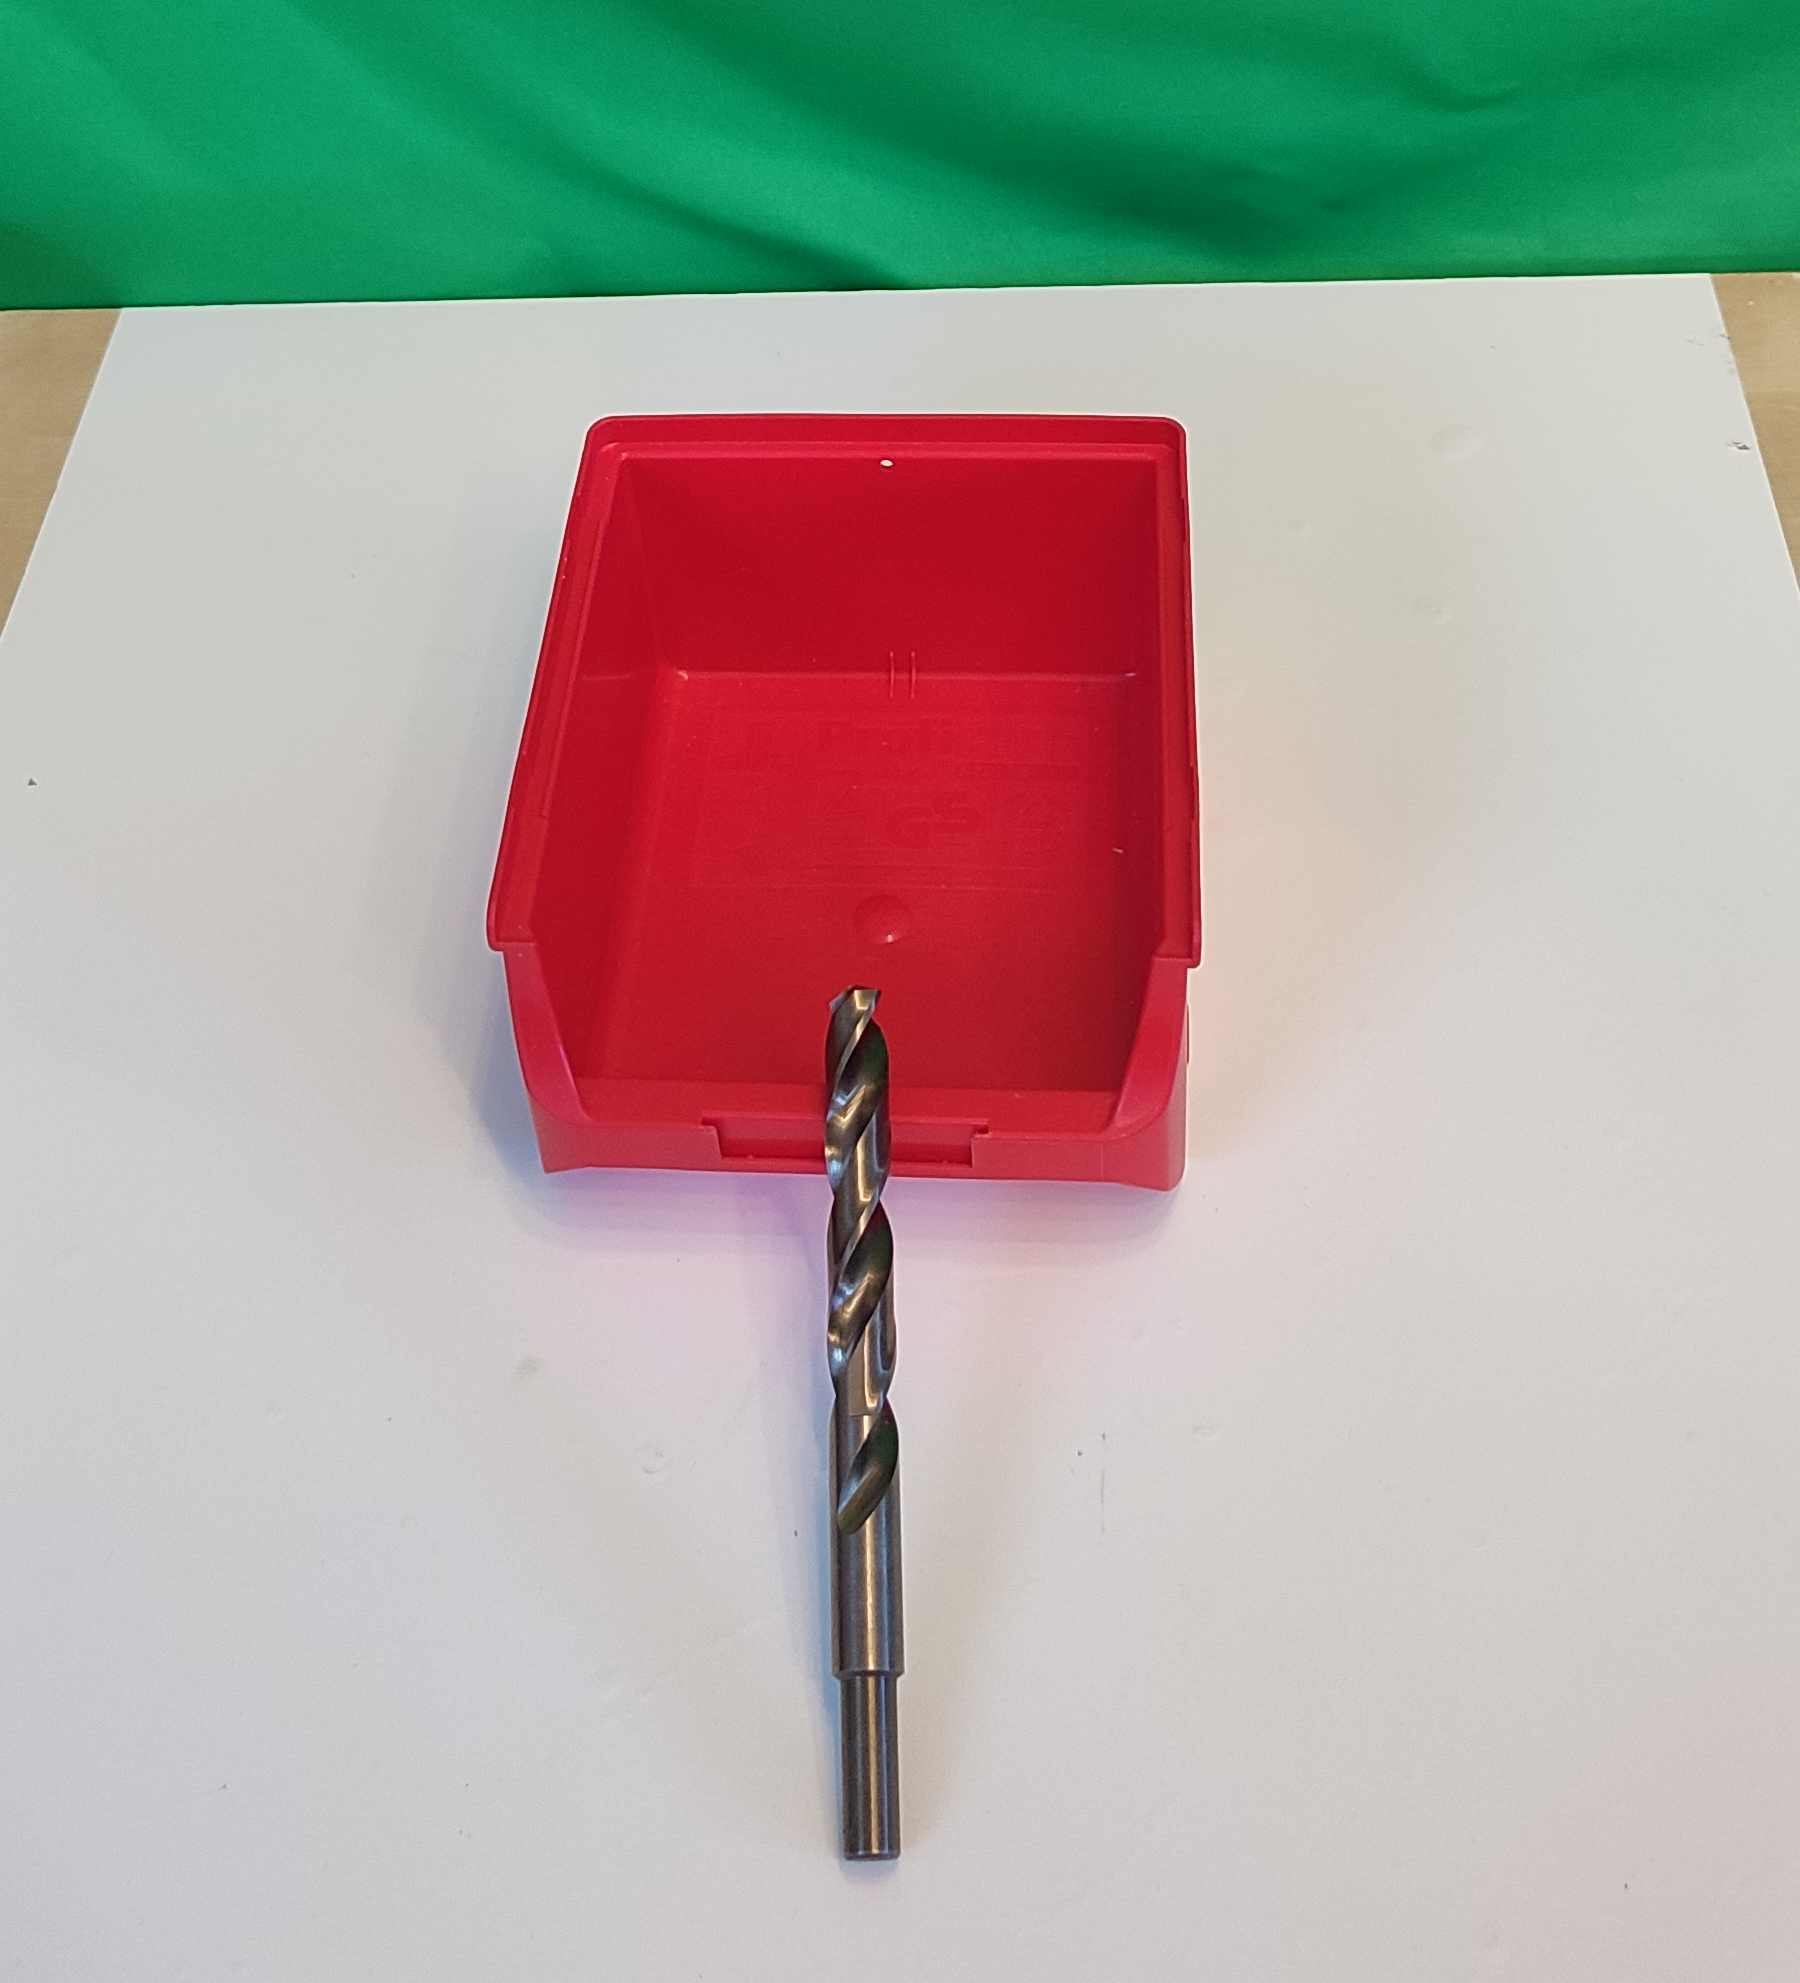
\includegraphics[width=0.24\textwidth,rotate=-0]{./images/placement_examples/drill_not_ok4.jpg}} \hfill	
\end{center}
	\caption{Examples of incorrect AllenKey and Drill  in container placement.}
	\label{fig:example_allenkeyNOTOK}
\end{figure}

If more than one object must be placed inside the same container, those objects are allowed to touch. 
The placement of the second object is also considered successful if the object does not touch the container bottom, 
if it is blocked by the first object (e.g. two large aluminum profiles into the same container) and its final position complies with the examples shown in fig. \ref{fig:example_allenkeyOK} without causing the mistakes shown in fig. \ref{fig:example_allenkeyNOTOK}.


\newpage
%% !TEX root = ../Rulebook.tex
\newpage
\section{Basic Navigation Test}

\paragraph{Purpose and Focus of the Test}
The purpose of the \iaterm{Basic Navigation Test}{BNT} is to check whether the robots can navigate well in their environment, i.e. in a goal-oriented, autonomous, robust, and safe way.
\par
As the navigation problem is in the focus of robotics research for a long time and many approaches for solving it and its subtasks (like exploration, mapping, self-localization, path planning, motion control, and obstacle avoidance) exist, the focus of this test is to demonstrate that these approaches function properly on the robots used by the teams and in the environment defined by the test.
\par

\paragraph{Scenario Environment}
The arena used for this test contains all elements that affect or support navigation: walls, service areas, places, arena objects, wall markers, and floor markers. In addition, obstacles may be placed in the environment.

\paragraph{Manipulation Objects}
This test does not include any objects for manipulation.
\paragraph{Task}
The robot will be sent a task specification, which is a string containing a series of triples, each of which specifies a place, an orientation, and pause duration. The robot has to move to the places specified in the task string, in the order as specified by the string, orient itself according to the orientation given, cover a place marker, pause its movement for the time in seconds as specified by the pause length, and finally leave the arena to reach the final position.

The task specification consists of:

\begin{itemize}
	\item[--] A destination location, e.g. \texttt{WS01}, \texttt{SH02}, \texttt{CB03} or \texttt{WP12}
	\item[--] An orientation (\texttt{N}, \texttt{S}, \texttt{W}, \texttt{E})
	\item[--] A duration in seconds
\end{itemize}

The duration is always set to 3 seconds in order to make validation easier for the referees.
%
% \subsection{Complexity Options}
%
% \subsubsection{Obstacle complexity (pick one):}
%
% \begin{itemize}
% 	\item Easy obstacles (bonus factor = +0.2): There are up to two obstacles in the arena.
% 	\item Medium obstacles (bonus factor =  +0.4): There are up to three obstacles in the arena and the placement of the obstacles is harder.
% \end{itemize}
%
%
% \subsubsection{Barrier Tape complexity (bonus factor = +0.4):}
% There are up to two barrier tape obstacles in the arena.
%
% \subsubsection{Navigation complexity (pick one):}
%
% \begin{itemize}
% 	\item Easy navigation (bonus factor = + 0.0): The place marker has to be covered in such a way by the robot that at least a part of the black area covered
% 	\item Medium navigation (bonus factor = + 0.1): The place marker has to be covered in such a way by the robot that at least a small part of the black area is covered the orientation must be correct, i.e. the robot must not deviate more than 45 deg.
% 	\item Hard navigation (bonus factor = + 0.2): The place marker has to be fully covered by the robot the orientation must be correct, i.e. the robot must not deviate more than 45 deg.
% \end{itemize}
%
%
\paragraph{Rules}
The following rules have to be obeyed:

\begin{itemize}
\item A single robot is used.
\item The robot has to start from outside the arena, enter it through the arena entrance and leave through the exit.
\item The order in which the teams have to perform will be determined by a draw.
\item After the team's robot enters the arena, it must move to the places given in the task specification and assume the orientation specified after the place. The robot may reach a destination by choosing any path.
\item The robot must visit the places in the order given by the task specification. It is possible to skip a place of the task specification and continue with the next one. In cases where the robot skipped one or multiple places there may be multiple possible matchings between places reached and places specified. In that case for calculating scores the matching is taken which leads to the highest score for the team.
\item A destination is counted as reached when the robot covers the place marker for the number of seconds specified by the break and does not move (very small movement of the wheels is allowed). The orientation must not deviate more than 45 degrees.
\item The run is over when the robot reached the final place or the designated time has expired.
\end{itemize}
%
%
%
% \subsection{Scoring}
%
% \begin{itemize}
% \item The team will receive 50 points for reaching a destination correctly (place and orientation) as given in the task specification and provided it stops for the time specified.
% \item The team receives a penalty of –50 points each time the robot touches an obstacle, a wall, an arena object or a service area (i.e. any contact with the environment).
% \item 50 points are awarded for completing the task specification completely correct, i.e. visiting all destinations from the task specification according to position and orientation (according to the chosen complexity level) and finally leaving the arena.
% \item The reached points of a test will be multiplied with the complexity factor that belongs to the chosen complexity level.
% \end{itemize}


% !TEX root = ../Rulebook.tex


\section{New Test Structure}
\label{sec:New Test Structure}

For the 2023 season, the TC decided to restructure the benchmark tests.
The main changes include:

\begin{itemize}
\item The dedicated test slots for "Precise Placement" and "Rotating Table" were removed. 
PP and RT were included in the more advanced tests.
\item As this removes two competition slots from the schedule and therefore leaves some "free time", one additional transportation task was added.
\item The now four total transportation tasks were split into two categories: "basic" and "advanced".
\item The requirements for all "basic" tasks (BMT, BTT1 \& BTT2) were relaxed in order for them to suit the naming.
\end{itemize}

We think that this had the following effects:

\begin{itemize}
\item The complexity of each test now increases more linear over the competition.
\item Teams with less experience should be able to successfully participate in the competition for longer rather than coming out of a test with no points.
\item Perfect runs are more achievable (for experienced teams) in the beginner tasks,
 bringing back more relevance to bonus points for reliable and consistent performance.
\end{itemize}



\section{Basic Manipulation Test (BMT)}

\subsection{Purpose and Focus of the Test}
The purpose of the Basic Manipulation Test is to demonstrate basic manipulation capabilities by the robots, like grasping, turning, or placing an object.
\par
The focus is on the manipulation and on demonstrating safe and robust grasping and placing of objects of different size and shape. Therefore, only minimal movement of the robot is required. 
\par
Some minor movement is intentionally designed into this test in order to force the teams to do dynamic assessment of the situation (e.g. estimating positions of manipulation objects, determining grasp positions, etc.) and to avoid that solutions depending on completely known initial situations and well-calibrated systems are possible. 

\subsection{Scenario Environment}
The arena used for this test contains basically all elements as for the Basic Navigation Test. Additionally to environmental elements (walls, service areas, floor markers, etc.), different manipulatable objects will be placed on the service areas. 

\subsection{Manipulation Objects}
The manipulation objects in this test include the objects specified in Table \ref{tab:manipulation_objects}.

\subsection{Task}
A single robot is used. The robot can be placed in an arbitrary starting location by the team. The task consists of a sequence of grasp and place operations, with a small base movement in between. The objective is to move a set of objects from one service area into another. The task is finished once all objects are moved or when the time foreseen for the run ends. 
\par
The task specification consists of: 
\begin{itemize}
	\item The specification of the initial place (e.g. D0, S5, U2)
	\item A source location, given as place (any one)
	\item A destination location, given as place (any one, but nearby the source location)
The specification of a final place for the robot (which does not need to be reached)
\end{itemize}

For now, in the competitions only the line is just as possible configuration:
\par
Line( \textless sequence of objects\textgreater )
\par
Further configurations may be specified in the future. Note, that the pose and orientation of each object in the destination service area is left unspecified and can be chosen by the robot. That means also objects don’t have to be put in a line.

Two examples for a full task specification is as follows:
\begin{itemize}
	\item BMT\textless S6,S6,S7,line(V20,R20,F20\_20\_B),S7\textgreater 
	\item BMT\textless S6,S6,S7,line(F20\_20\_G,F20\_20\_B,M20\_100),S7\textgreater 
\end{itemize}


\subsection{Complexity Options}

\subsubsection{Manipulation Object complexity (pick one):}

\begin{itemize}
\item Choose objects (bonus factor =  0.0): The team can freely choose the manipulation objects.
\item Few objects (bonus factor =  0.2): The team can freely choose a set of five manipulation objects.
\item All objects (bonus factor =  0.5): All manipulations objects can be used.
\end{itemize}


\subsubsection{Decoy Object complexity (pick one):}

\begin{itemize}
\item No decoy objects (bonus factor =  0.0): No decoy objects will be used.
\item Few decoy objects (bonus factor =  0.2): The team can freely choose a set of three manipulation objects, to be used as decoy.
\item All decoy objects (bonus factor =  0.3): All manipulations objects can be used as decoy.
\end{itemize}


\subsubsection{Orientation Complexity (bonus factor = 0.2):}
The manipulation objects can be placed in all orientations.

\subsubsection{Rotation Complexity (bonus factor = 0.2):}
The manipulation objects can be placed in all orientations.

\subsubsection{Position Complexity (bonus factor = 0.2):}
The manipulation objects while be placed by the referees.

\subsection{Rules}
The following rules have to be obeyed:

\begin{itemize}
\item The order in which the teams have to perform will be determined by a draw.
\item A team has a time period of 5 minutes to complete a run.
\item At the beginning of a team’s period, the team will get the task specification. 
\item The team can setup the robot anywhere inside the arena.
\item A manipulation object counts as successfully grasped as defined in Section 5.5.3.
\item A manipulation object counts as successfully placed, if the robot has placed the object into the correct destination service area as described in Section 5.5.4.. 
\item The team has at most 5 minutes to complete the task. The time is stopped when the robot has completed task by placing the last object of the task specification. If a team cannot complete the task within 5 minutes, the run will be stopped after 5 minutes. 
\end{itemize}


\subsection{Scoring}
Points are awarded as follows:

\begin{itemize}
\item 100 points are awarded for successfully grasping a manipulation object that is part of the task specification..
\item 50 points are awarded for successfully placing a manipulation object into the destination service area.
\item - 100 points for grasping a wrong manipulation object.
\item 50 points are awarded for completing the task specification completely correct. 
\item The reached points of a test will be multiplied with a defined complexity factor depending on the previously chosen complexity level.
\end{itemize}



% !TEX root = ../Rulebook.tex

\section{Basic Transportation Test}
\label{sec:Basic Transportation Test}

The \iaterm{Basic Transportation Test}{BTT} targets both navigation and manipulation, aswell as logistical optimization. Objects are initially placed on randomly selected service areas and must be transported to their specific target location.
As their total number now exceeds the inventory size, robots will have to manage their inventory content and optimize their payload. The object pool consists of the complete Basic Object Set.

There are currently two versions of the BTT. 
They gradually introduce more elements of the league to the competition, including the randomness of the used objects, the increase of active Service Areas and them not being next to each other anymore, using different table heights and the placement of physical obstacles.

The following paragraphs summarize the two different levels but DO NOT override the test specification in table \ref{fig:test_specifications_instance}.

\paragraph{BTT1}
\begin{itemize}
\item Four randomly selected objects have to be transported.
\item There will be three active service areas and they are not next to each other.
\item Only tables with a height of 10cm are used. 
\end{itemize}

\paragraph{BTT2}
\begin{itemize}
\item Five randomly selected objects have to be transported.
\item Two randomly selected decoy objects are placed onto one or more randomly selected service areas.
\item There will be four active service areas with each covering one of the four table heights (0, 5, 10, 15 $\si{\centi\meter}$).
\item Physical Obstacles are placed inside the arena (one blocking, one semi-blocking).
\end{itemize}

% !TEX root = ../Rulebook.tex

\section{Advanced Transportation Test}
\label{sec:Advanced Transportation Test}

The \iaterm{Advanced Transportation Test}{ATT} has its origins as a BTT, but greatly increases the difficulty of the tasks to perform by introducing more random elements. 

This includes the introduction of arbitrary surfaces, shelfs and precise placement tables, barriertape as visual obstacles and the containers as target objects. With the object count further increasing, task optimization and replanning in case of failure also becomes more relevant.

As with the BTTs, there are two versions of the ATT, which gradually introduce the more challenging elements of \RCAW.
The following paragraphs summarize the two different levels but DO NOT override the test specification in table \ref{tab:Instances}.

\paragraph{ATT1}
\begin{itemize}
\item Six randomly selected objects have to be transported.
\item Three randomly selected decoy objects are placed onto one or more randomly
\item There will be five active service areas (four tables and one shelf)
\item All table heights are used (0-15 $\si{\centi\meter}$).
\item Two Objects must be placed on a shelf (top part).
\item Virtual Obstacles (Barriertapes) are placed inside the arena (one blocking, one non-blocking).
\item Two service areas will have an arbitrary surface.
\end{itemize}

\paragraph{ATT2}
\begin{itemize}
\item Seven randomly selected objects have to be transported.
\item Five randomly selected decoy objects are placed onto one or more randomly
\item There will be six active service areas (four tables,  one shelf and one Precise Placement table)
\item All table heights are used (0-15 $\si{\centi\meter}$).
\item One object must be picked from a shelf (lower part).
\item One object must be Precise Placed.
\item Two objects must be placed into a container (preferably one to each color).
\item One visual and one physical obstacle is placed inside the arena (both semi-blocking).
\item Three service areas will have an arbitrary surface.
\end{itemize}

%\newpage
\section{Precision Placement Test}
\label{sec:Precision Placement Test}

\paragraph{Purpose and Focus of the Test}
The purpose of the \iaterm{Precision Placement Test}{PPT} is to assess the robot's ability to grasp and place objects into object-specific cavities. This demands advanced perception abilities (to recognize the correct cavity for each object) and manipulation abilities (to grasp and place the object in such a manner that it fits into the cavity).

\paragraph{Scenario Environment}
The same arena as for the Basic Manipulation Test is used. In case that the arena does not already include a modified service area as shown in Figure \ref{fig:ppt_plattform}, it will be added only for this particular test. The modified service arena includes object-specific cavities as shown in the Figure~\ref{fig:ppt_tiles}. For each object used in the test, there will be one specific cavity. The cavity has the dimension of the object plus a 2 mm offset for each dimension. At most five cavities are used in the test.


\begin{figure} [h!]
\begin{center}
\subfloat[F20\_20]{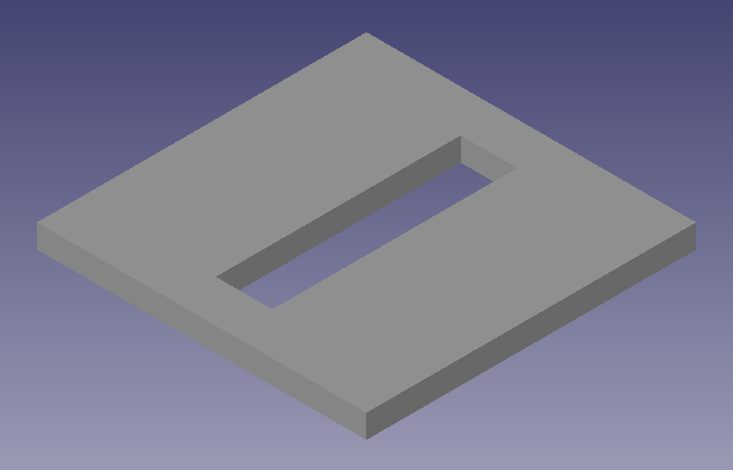
\includegraphics[width = 2cm]{./images/ppt_F20.png}} \hspace{0.1cm}
\subfloat[S40\_40]{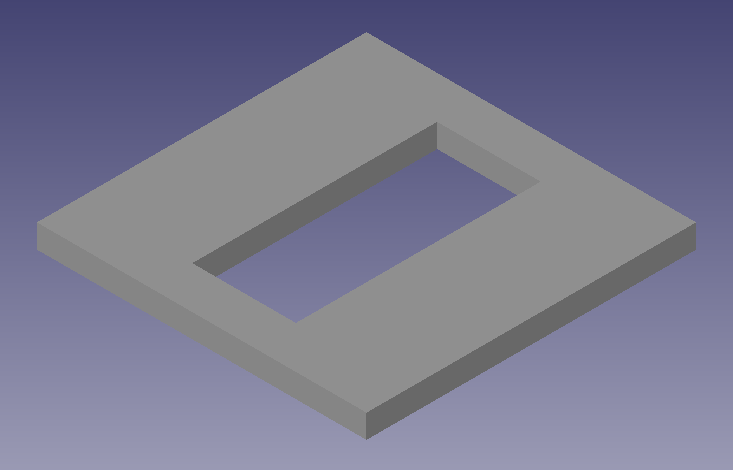
\includegraphics[width = 2cm]{./images/ppt_S40.png}} \hspace{0.1cm} 
\subfloat[M20\_100]{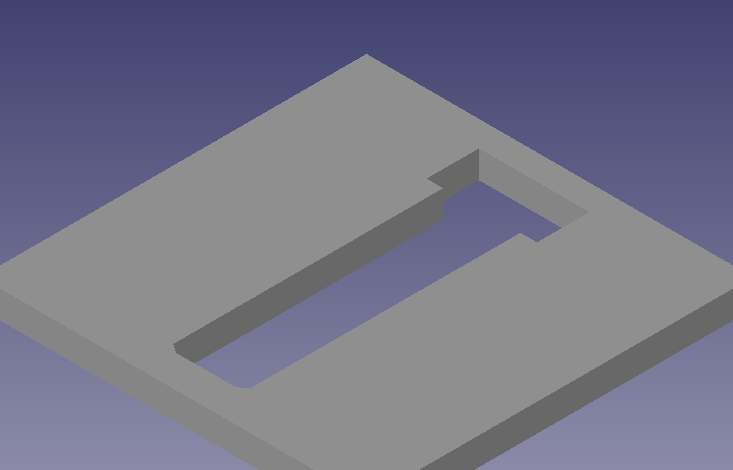
\includegraphics[width = 2cm]{./images/ppt_M20_100.png}}  \hspace{0.1cm}
\subfloat[M20]{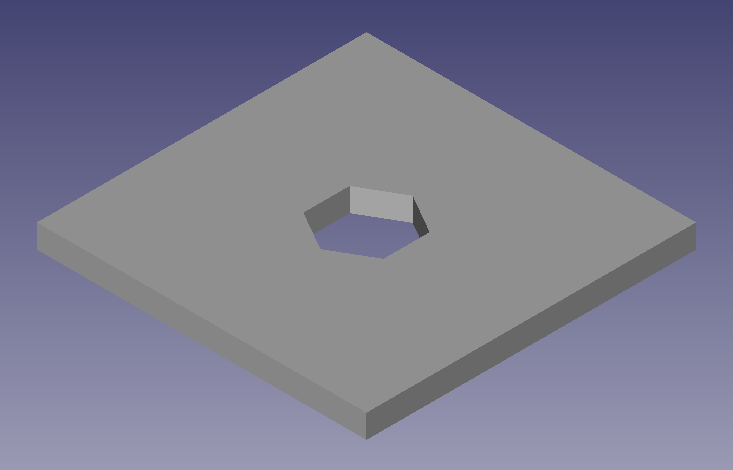
\includegraphics[width = 2cm]{./images/ppt_M20.png}}  \hspace{0.1cm}
\subfloat[M30]{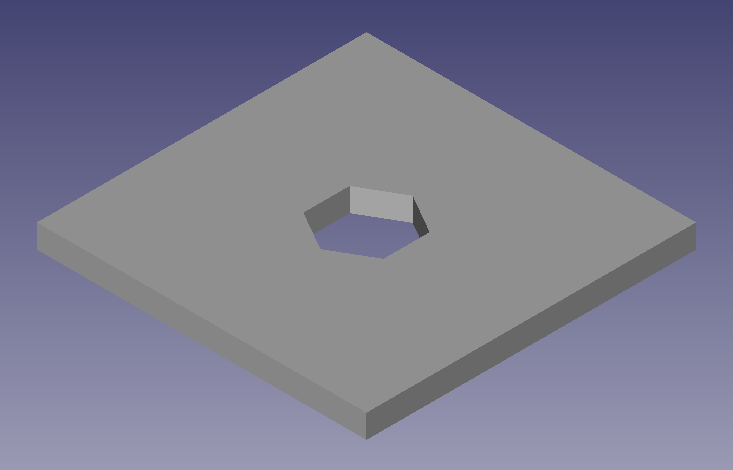
\includegraphics[width = 2cm]{./images/ppt_M30.png}}  \hspace{0.1cm}
\subfloat[R20]{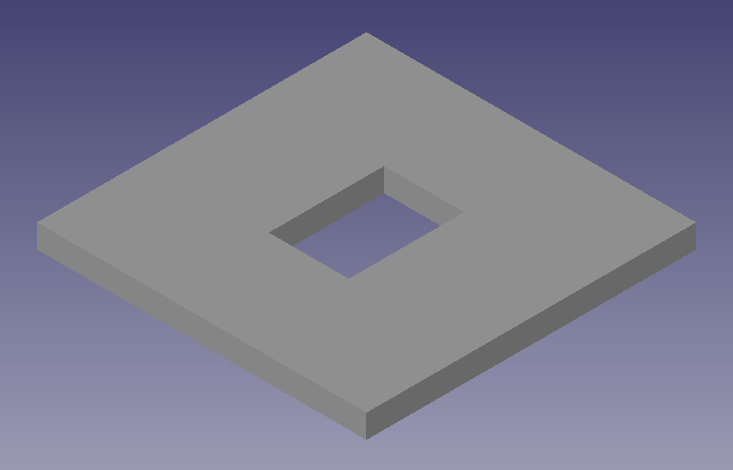
\includegraphics[width = 2cm]{./images/ppt_VR20.png}} \\
\subfloat[F20\_20]{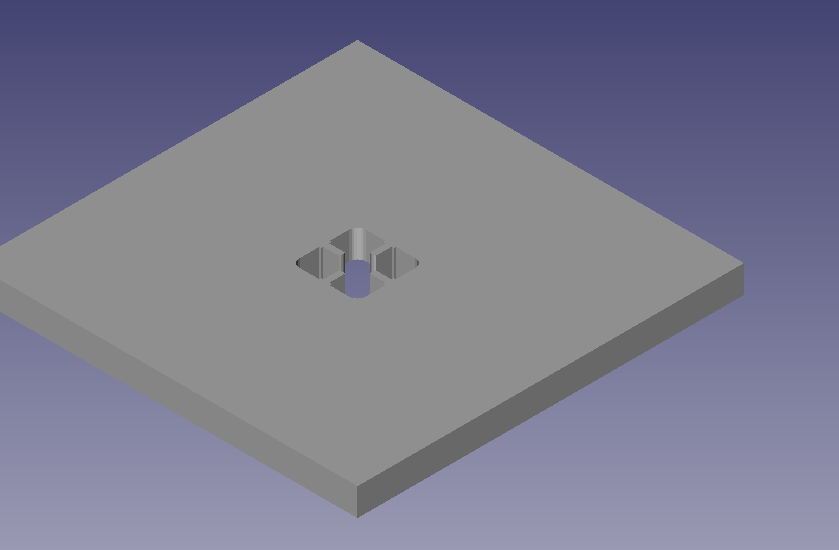
\includegraphics[width = 2cm]{./images/ppt_F20_v.png}}  \hspace{0.1cm}
\subfloat[S40\_40]{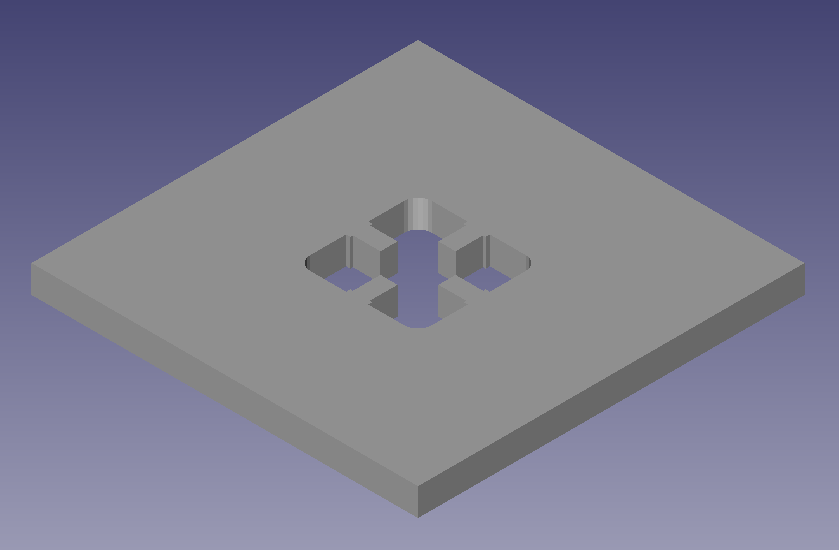
\includegraphics[width = 2cm]{./images/ppt_S40_v.png}}   \hspace{0.1cm}
\subfloat[M20\_100]{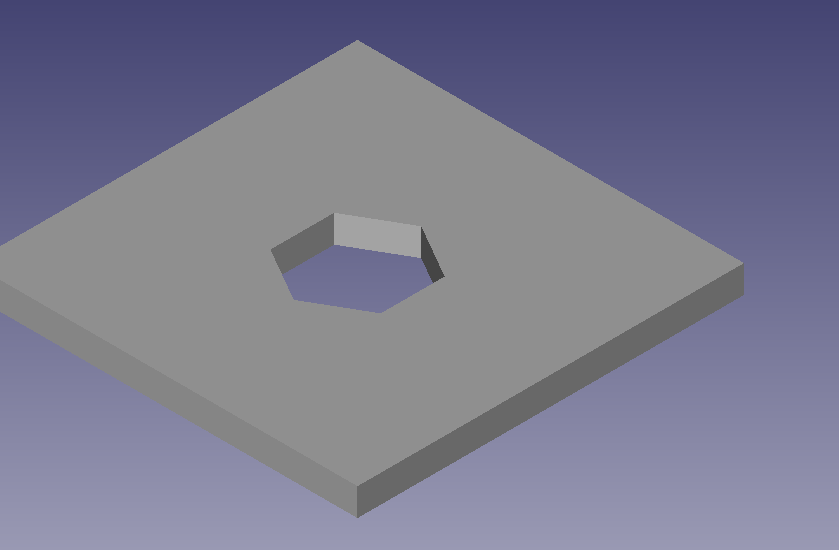
\includegraphics[width = 2cm]{./images/ppt_M20_100_v.png}} \hspace{0.1cm}
\subfloat[M20]{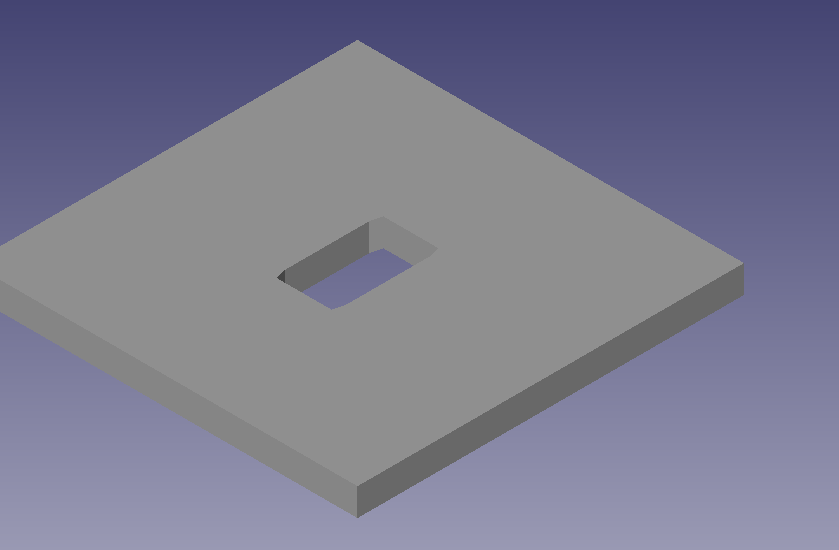
\includegraphics[width = 2cm]{./images/ppt_M20_v.png}}  \hspace{0.1cm}
\subfloat[M30]{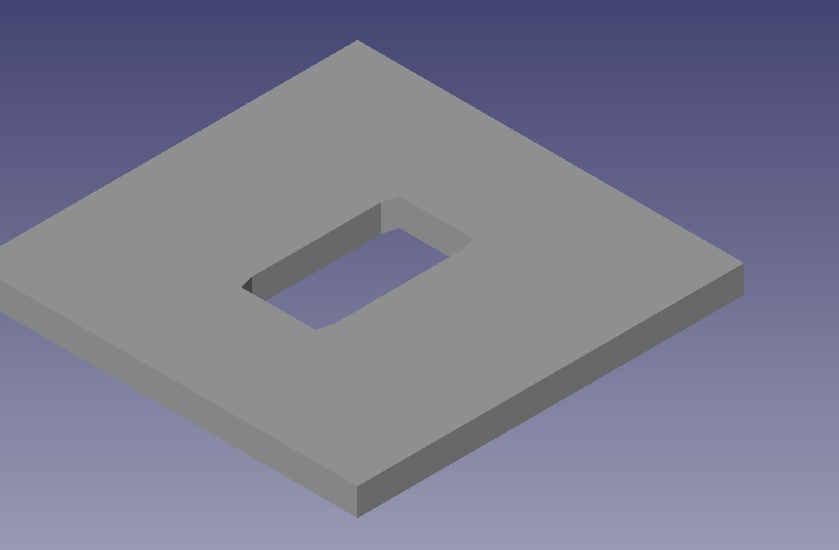
\includegraphics[width = 2cm]{./images/ppt_M30_v.png}}  \hspace{0.1cm}
\subfloat[R20]{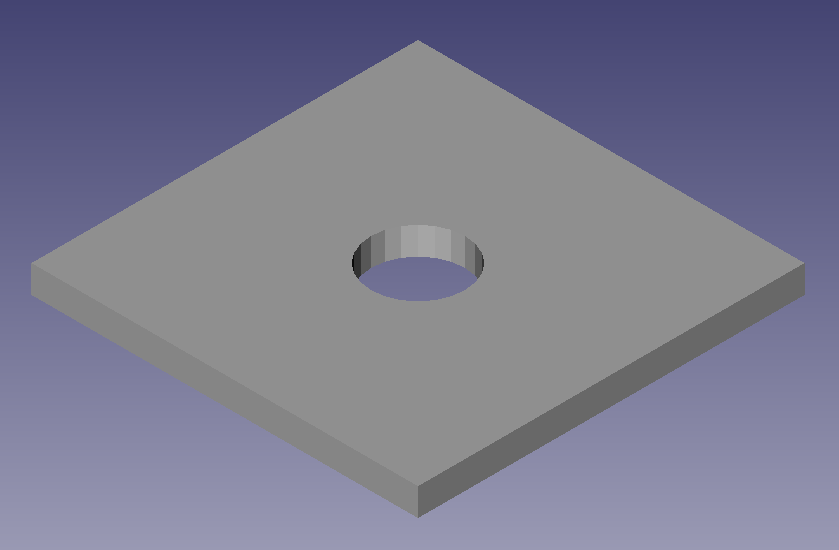
\includegraphics[width = 2cm]{./images/ppt_VR20_v.png}} 
\end{center}
\caption{Illustration of horizontal (top row) and vertical (bottom row) cavities for the different kind of manipulation objects.}
\label{fig:ppt_tiles}
\end{figure}


\paragraph{Manipulation Objects}
The manipulation objects used in this test are defined by the instances described in Table~\ref{tab:Instances}.

\paragraph{Task}
The objective of the task is to pick the objects which are placed on one service area and make a precise placement in the corresponding cavity at the service area with the special PPT platform (an example configuration is illustrated in Figure \ref{fig:ppt_plattform}). 

\begin{figure}
\centering
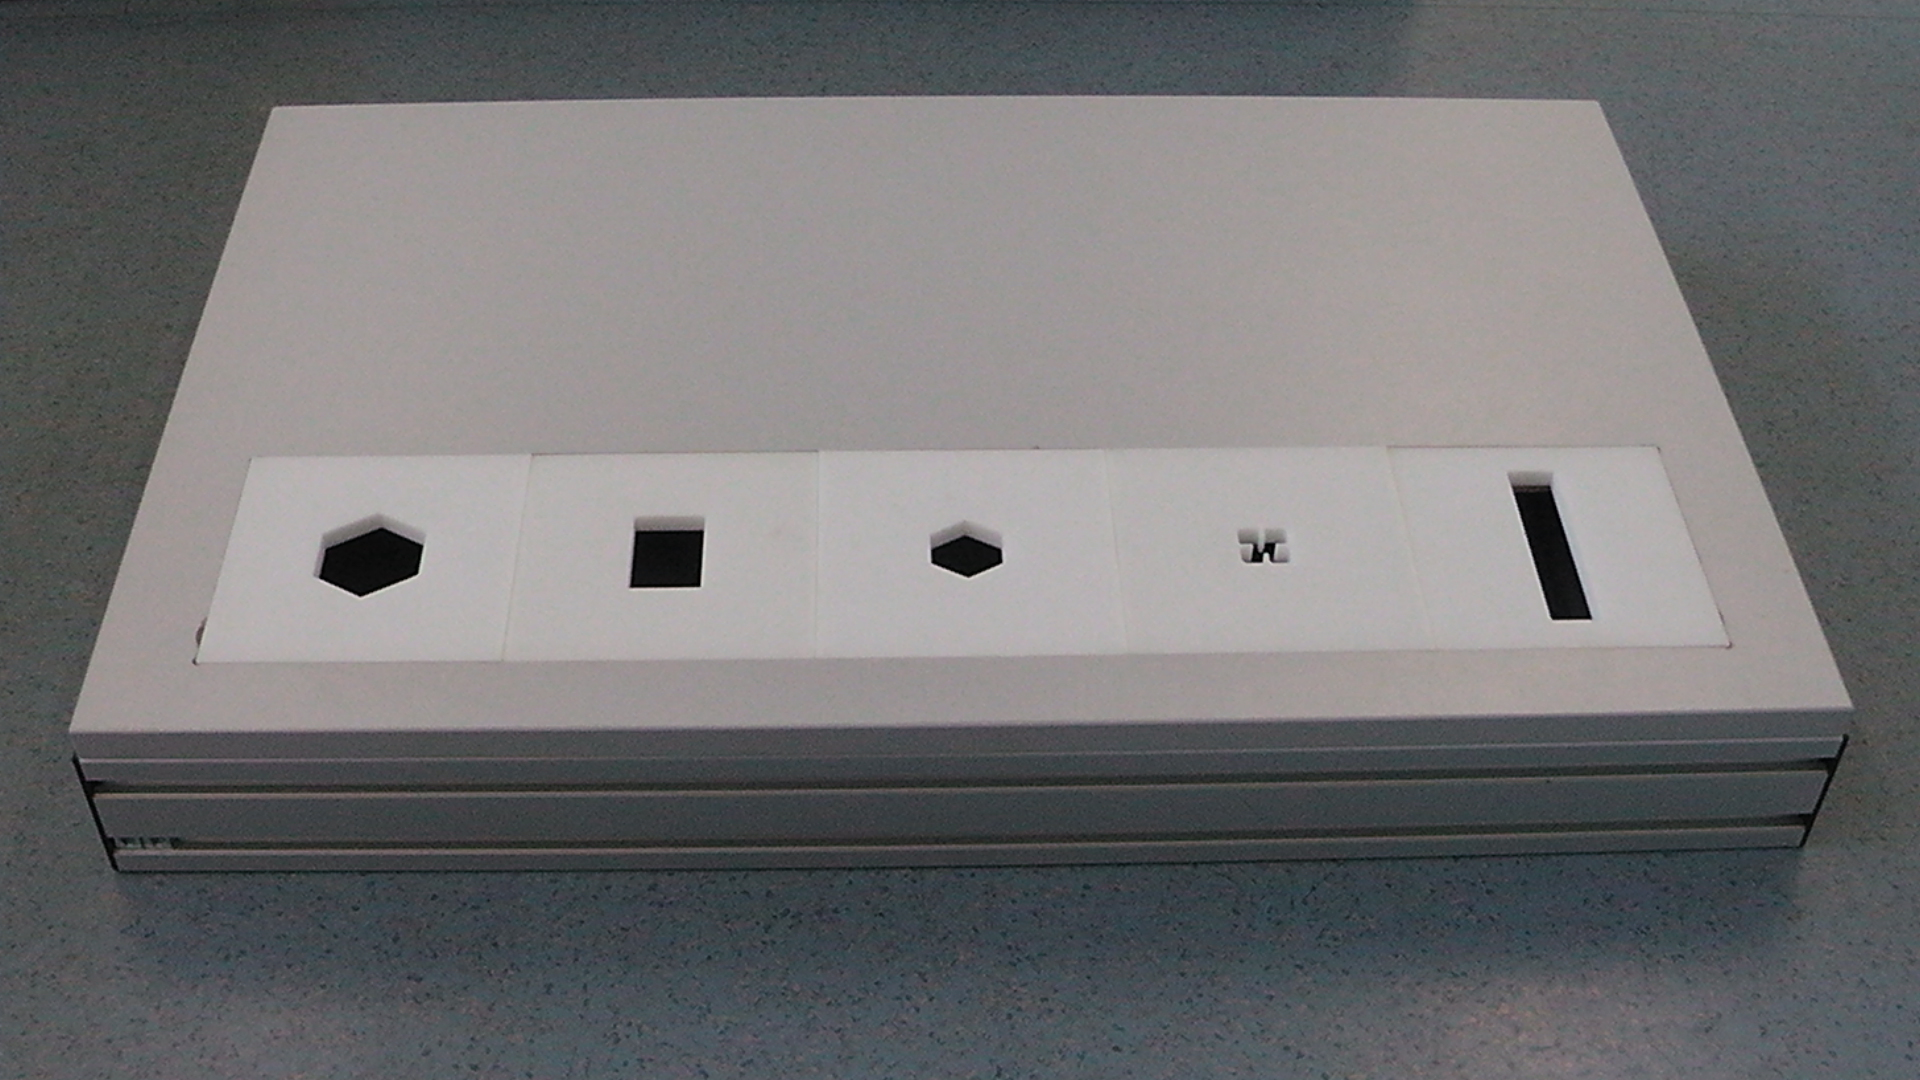
\includegraphics[width=0.6\textwidth ]{./images/ppt_plattform.jpg}
\caption{The PPT platform including five cavity tiles}
\label{fig:ppt_plattform}
\end{figure}

The task consists of multiple grasp and place operations, possibly with base movement in between, which will, however, be short. Note that the placement of the object in the cavity is finished when the object is fallen into the cavity (i.e. at least some part of the object has to touch ground floor underneath the cavity).

%
%\subsection{Complexity Levels}
%
%All Complexity Options from BMT apply.
%
%\subsubsection{PPT Orientation Complexity (bonus factor = 0.2):}
%The cavities can be placed in all orientations.
%\subsubsection{PPT Rotation Complexity (bonus factor = 0.2):}
%The cavities can be placed in all orientations.

\paragraph{Rules}
The following rules have to be obeyed:

\begin{itemize}

\item A single robot is used.
\item The robot has to start from outside the arena and to end in the final.
\item The order in which the teams have to perform will be determined by a draw.
\item The robot will get the task specification from the referee box.
\item A service area counts as successfully reached as defined in Section~\ref{ssec:Navigating}.
%\item A manipulation object counts as successfully grasped as specified in Section~\ref{ssec:GraspingObjects}.
\item An object counts as placed correctly if it fell through the correct cavity and touches the ground beneath. It may happen that an object blocks the cavity for the next object, e.g. by standing upright on the floor. In that case a referee may remove that object (which remains to count as a successful place). If the referee is not able to do so and the robot places another object into the blocked cavity, it counts as a correct placement if it would have been successful without the blocking object.
\item The run is over when the robot reached the final position or the designated time has expired.
\item The score for this test will be calculated as defined in \ref{sec:ScoringAndRanking}.

\end{itemize}

%\subsection{Scoring}
%Points are awarded as follows:
%
%\begin{itemize}
%\item 50 points are awarded for successfully grasping an object.
%\item 100 points are awarded for successfully placing a manipulation object into the correct cavity.
%\item 50 points are awarded if the task specification has been completely fulfilled. The task is considered as fulfilled if all objects have been dropped in the right cavity. The robot does not have to leave the arena.
%\item a penalty of -50 points is given for each object which has been dropped into the wrong cavity
%\item The reached points of a test will be multiplied with a defined complexity factor depending on the previously chosen complexity level.
%\end{itemize}




%% !TEX root = ../Rulebook.tex
%\newpage
\section{Rotating Table Test}
\label{sec:Rotating Table Test}

The \iaterm{Rotating Table Test}{RTT} introduces moving objects to the competition.
A total of six objects are placed on the rotating table (\Marco{add ref to arena design, special rtt}), of which three must be picked and three are decoy objects.

This requires robots to detect objects and estimate their trajectory in order to grasp them successfully.
To lower the difficulty of this task, the table continously spins with a constant speed, enabling robots to use data from multiple rotations to calculate the optimal grasping position and move their manipulator in time.

It is explicitly NOT allowed to stop the table (e.g. by pushing the gripper into the table surface).
It is also explicitly NOT allowed to position the gripper in a way that blocks the objects 
unless it is during the grasping process of a target object and does not affect the table rotation or other objects.

The table starts spinning once the runtime of each team has started.
The initial table rotation is the same for each team to ensure comparability.  

As navigation is not the focus of this test, robots only have to travel to the rotating table and do not have to move to the FINISH location. The run ends once all three objects have been picked or a rule violation has been called by the referees.



%
%\paragraph{Purpose and Focus of the Test}
%The purpose of the \iaterm{Rotating Table Test}{RTT} is to assess the robot's ability to manipulate moving objects which are placed on a rotating turntable. The test demands fast perception and manipulation skills in order to pick up objects from a moving surface.
%
%\paragraph{Scenario Environment}
%The same arena as for the Basic Manipulation Test is used. In case that the arena does not already include such a device (see Figure \ref{fig:conveyor_belt}), it will be added only for this particular test.
%
%\begin{figure} [h!]
%	\begin{center}
%%		\subfloat[Conveyor belt]{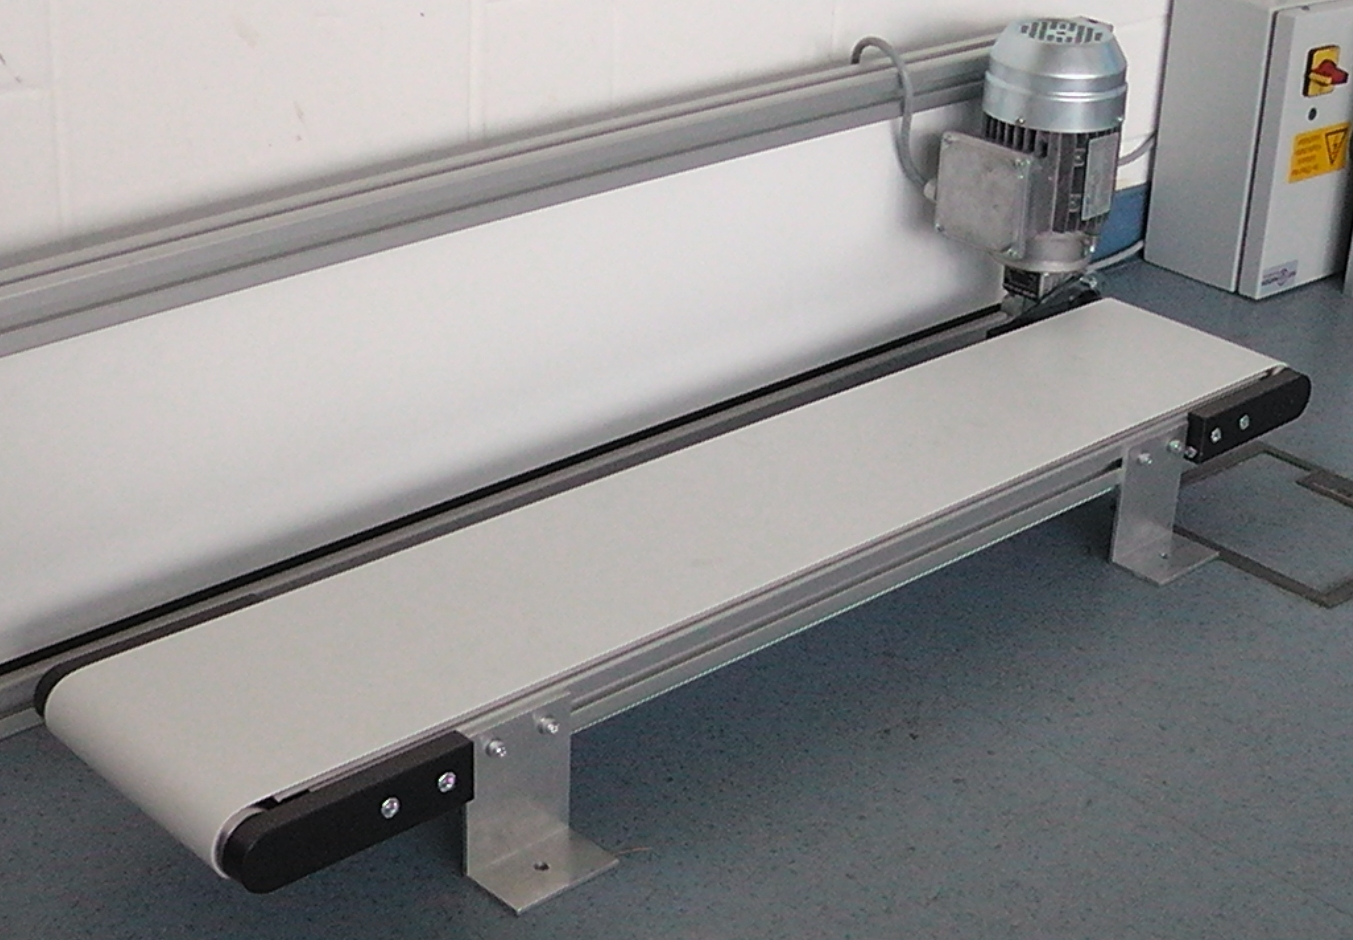
\includegraphics[height = 4cm]{./images/conveyor_belt.jpg}} 
%%		\hspace{1cm}
%		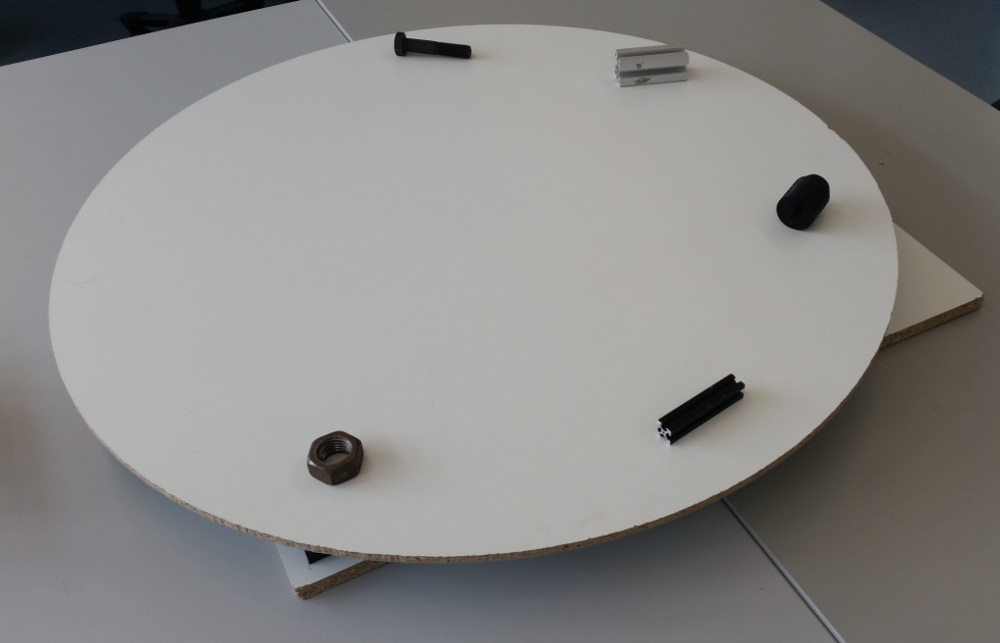
\includegraphics[height = 6cm]{./images/rotating_table.jpg}
%	\end{center}
%	\caption{Illustration of a rotating table used in the competition.}
%	\label{fig:conveyor_belt}
%\end{figure}
%
%
%
%\paragraph{Manipulation Objects}
%The manipulation objects used in this test are defined by the instances described in Table~\ref{tab:Instances}.
%
%\paragraph{Task}
%The task of the robot is to navigate to the location of the rotating table and to grasp all objects from the moving table. The objects can pass multiple times in front of the robot, until the maximum time for the run is over. The robot is supposed to place the grasped objects on the robot itself.
%
%
%%\subsection{Complexity Options}
%%All Complexity Options from BMT apply.
%
%
%%\subsubsection{Speed Complexity (pick one):}
%%
%%\begin{itemize}
%%\item low speed (bonus factor = +0.0): The conveyor belt speed will be not more than 0.5 cm/s
%%\item medium speed (bonus factor = +02):	The conveyor belt speed will be not more than 0.75 cm/s
%%\item high speed (bonus factor = +0.4): The conveyor belt speed will be not more than 0.10 cm/s
%%\end{itemize}
%
%
%
%\paragraph{Rules}
%The following rules have to be obeyed:
%
%\begin{itemize}
%\item A single robot is used.
%\item The robot has to start from outside the arena and to end in the final.
%\item The order in which the teams have to perform will be determined by a draw.
%\item The objects are placed on the rotating table before the run starts by the OC or TC.
%\item The speed of the rotating table is determined by the OC or TC just before the test starts.
%\item The robot will get the task specification from the referee box.
%\item A service area counts as successfully reached as defined in Section~\ref{ssec:Navigating}
%\item A manipulation object counts as successfully grasped as specified in Section~\ref{ssec:PlacingObjects}.
%\item The objects have to be grasped actively from the moving table. The robot is not allowed to stop the items with its gripper.
%\item The run is over when the robot reached the final position or the designated time has expired.
%\item The score for this test will be calculated as defined in \ref{sec:ScoringAndRanking}.
%\end{itemize}
%
%
%
%%
%%\subsection{Scoring}
%%Points are awarded as follows:
%%
%%\begin{itemize}
%%\item 200 points are awarded for successfully grasping an object from the conveyor belt 
%%\item -150 points are given if an object dropped onto the ground, is placed not on the robot itself or dropped from the end of the conveyor..
%%\item -100 points are given if the referees had to switch on the belt manually after signalled by a team member, while a working automatic wireless mechanism to switch it on was available.
%%\item 50 points are awarded if the task has been fully achieved (when all objects placed on the belt are grasped).
%%\end{itemize}


\section{Final}
\label{sec:Final}

The \iaterm{Final Run}{Final} acts as the full benchmark for robots, including all elements of \RCAW.
With the number of objects and active service areas at its peak, task planning and execution speed may become a limiting factor for competing robots. The following paragraph summarizes the final, but DOES NOT override the test specification in table \ref{fig:test_specifications_instance}.

\paragraph{Final}
\begin{itemize}
\item Ten randomly selected objects have to be transported.
\item Eight randomly selected decoy objects are placed onto one or more randomly selected (active) service areas
\item There will be eight active service areas (four tables,  two shelfs, one Rotating Table and one Precise Placement table)
\item All table heights are used (0-15 $\si{\centi\meter}$).
\item Two objects must be picked from a shelf (lower part).
\item Two objects must be picked from the Rotating Table.
\item Two objects must be placed on a shelf (top part).
\item Two objects must be placed in the Precision Placement Cavity.
\item Four objects must be placed into a container (two in blue, two in red).
\item Two visual and two physical obstacles are placed inside the arena (two blocking, one semi-blocking, one non-blocking).
\item Four service areas will have an arbitrary surface.
\end{itemize}

% !TEX root = ../Rulebook.tex
\section{Test Specification Summary}
\renewcommand{\arraystretch}{1.1}
\newcommand{\R}[2]{
	\begin{turn}{90}
		\begin{minipage}[][1em][c]{#2}
		#1
	  \end{minipage}
	\end{turn}
}
\newcommand{\cir}[1]{\hspace{0.5em}\unitlength1ex\begin{picture}(2.8,2.8)%
\put(0.75,0.75){\circle{2.8}}\put(0.75,0.75){\makebox(0,0){#1}}\end{picture}}
\newcommand{\Y}{\tiny \CIRCLE}
\newcolumntype{P}[1]{>{\centering\arraybackslash}p{#1}}

\definecolor{headlineColor}{rgb}{.7,.7,.7}
\definecolor{sectionColor}{rgb}{.7,.1,.1}

\newcommand{\C}{\cellcolor{sectionColor}}
%\begin{landscape}
%\begin{table}[h!]
% \centering
% \begin{tabular}{|l|l|l*{11}{|P{1cm}}|}
%   \hhline{~~~--------}
%   \multicolumn{3}{l|}{ }                   &  \multicolumn{8}{c|}{Instances}                        \\
%   \hhline{~~~--------}
%   \multicolumn{3}{l|}{ }                   &\cir{1}&\cir{2}&\cir{3}&\cir{4}&\cir{5}&\cir{6}&\cir{7} \\
%   \multicolumn{3}{r|}{ }                   & BMT   & BTT1  & BTT2  &  BTT3 &  PPT  &  RTT  & Final  \\
%   \hhline{~~~--------} \hline
%   \multirow{5}{0.5cm}{\R{\centering Objects}{3.0cm}}
%   & \RCAW \&  RoCKIn            & atwork-commander   & 5     & 5     & 6     & 6     & 3      & 3     & 10    \\ \hhline{~----------}
%   & Decoy                       & TC   &       & 3     & 3     & 3     &        & 3     & 5     \\ \hhline{~----------}
%	 & Position                    &          & Ref   & Ref   & Ref   & Ref   & Team   & Ref   & Ref   \\ \hhline{~----------}
%	 & Rotation                    &          & Team  & Ref   & Ref   & Ref   & Team   & Team  & Ref   \\ \hhline{~----------}
%	 & Orientation                 &          & Team  & Team  & Team  & Ref   & Team   & Team  & Ref   \\ \hline
%   \multirow{6}{0.5cm}{\R{\centering Service area}{3.5cm}}
%   & Estimated Active            & atwork-commander   & 2     & 3     & 4     & 5     & 2      & 1     & 8     \\ \hline
%   & Table height                & atwork-commander   &       &       & 0 cm  &       &        &       &  0 cm \\
%   &                             &          &       &       & 5 cm  &       &        &       &  5 cm \\
%   &                             &          & 10 cm & 10 cm & 10 cm & 10 cm &  10 cm & 10 cm & 10 cm \\
%   &                             &          &       &       & 15 cm &       &        &       & 15 cm \\ \hhline{~----------}
%	 & Arbitrary surface           & TC   &       & 1     & 2     & 2     &        &       & 3     \\ \hline
%	 \multirow{3}{0.5cm}{\R{\centering Arena }{1.5cm}}
%	 & Physical Obstacles          & TC  &       &       & 2     & 2     &        &       & 2     \\ \hhline{~----------}
%	 & Virtual Obstacles           & TC  &       & 2     &       & 1     &        &       & 2     \\ \hhline{~----------}
%   &                             &          &       &       &       &       &        &       &       \\ \hhline{-----------}
%   \multirow{3}{0.5cm}{\R{\centering Grasping }{1.64cm}}
%   & Shelf unit                  & atwork-commander   &       &       &       & 2     &        &       & 2     \\ \hhline{~----------}
%	 & Rotating table          & Referee  &       &       &       &       &        & 3     & 1     \\ \hhline{~----------}
%   & Rotating direction          &          &       &       &       &       &        & Team  & Ref   \\ \hline
%   \multirow{8}{0.5cm}{\R{\centering Placement}{2.5cm}}
%   & Preisicon placement table  & atwork-commander   &       &       &       &       & 3      &       & 1     \\ \hhline{~----------}
%   & Shelf unit                  & atwork-commander   &       &       &       & 1     &        &       & 1     \\ \hhline{~----------}
%   & Red container               & atwork-commander   &       &       &       & 2     &        &       & 2     \\ \hhline{~----------}
%   & Blue container              & atwork-commander   &       &       &       & 2     &        &       & 2     \\ \hhline{~----------}
%   & Rotating turntable          & atwork-commander   &       &       & 1     &       &        &       &       \\ \hhline{~----------}
%   & Cavities Position           &    &       &       &       &       & Ref	   &       & Ref   \\ \hhline{~----------}
%   & Cavities Rotation	         &  &       &       &       &       & Ref    &       & Ref   \\ \hhline{~----------}
%   & Cavities Orientation	       &   &       &       &       &       & Team   &       & Team  \\ \hline \hline
%   \multicolumn{2}{|l|}{Duration}
%                                 & atwork-commander   & 5min  & 6min  & 10min & 10min & 4min   & 4min  & 13min \\
% 		\hline
% \end{tabular}
% \caption{Test specification in the instances of the \RCAW \YEAR competition.}
% \label{tab:Instances}
%\end{table}


\begin{figure}[h!]
	\centering
	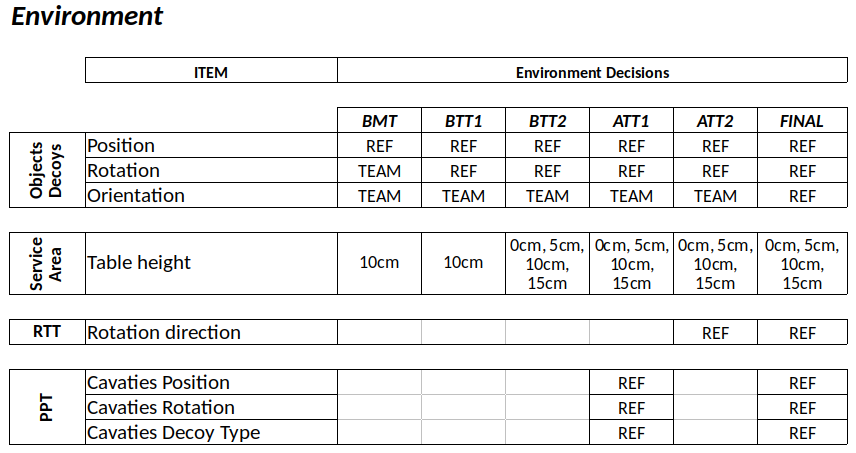
\includegraphics[width= 1.0\textwidth ]{./images/tabels/robocup_env.png}
	\caption{Test specification in the environment of the \RCAW \YEAR competition.}
	\label{fig:test_specifications_environment}
\end{figure}

\begin{figure}[h!]
	\centering
	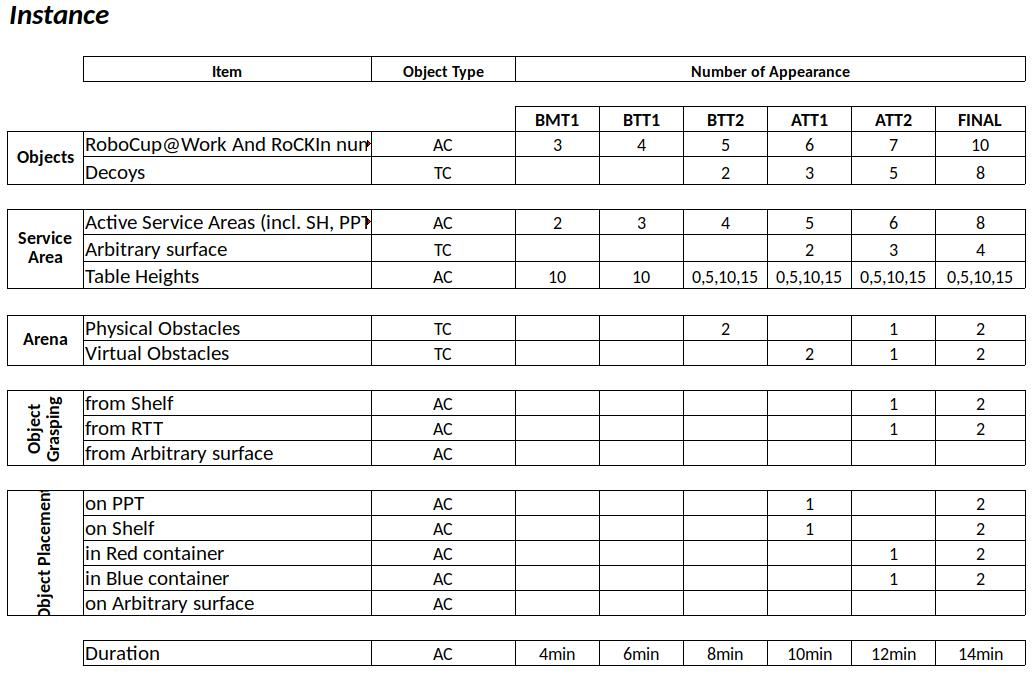
\includegraphics[width= 1.0\textwidth ]{./images/tabels/robocup_instance.jpg}
	\caption{Test specification in the instances of the \RCAW \YEAR competition.}
	\label{fig:test_specifications_instance}
\end{figure}
%\end{landscape}





%\newpage
%\section{Test Variability} \label{sec:TestVariability}

%The different optional parameters and configurations for each task are 
%mentioned in Section~\ref{sec:ArenaDesign} and \ref{sec:ManipulationTasks}. 
%Figure~\ref{fig:complexityTree} summarizes the possible variations and 
%emphasizes aspects that may be chosen.

%\begin{figure}[ht]
%\centering
%\tikzset{
  basic/.style  = {draw, rectangle, thin, text width=2cm, 
	                 rounded corners=2pt, align=center},
  root/.style   =  {basic},
  level 2/.style = {basic, sibling distance=45mm},
  level 3/.style = {basic, align=left},
  level 4/.style = {basic, align=left, fill = white!50, node distance = 0.7cm},
	box/.style = {draw, black, dashed}
}

\begin{tikzpicture}[
  font = \footnotesize,
  level 1/.style={sibling distance=70mm},
  edge from parent/.style={->,draw},
  >=latex]

% root of the the initial tree, level 1
\node[root] {Complexities}
% The first level, as children of the initial tree
  child {node[level 2] (c1) {Manipulation}
       child  {node[level 3]  (OBJECTS) {Objects}}
       child {node[level 3]  (GRASPING) {Grasping} }
       child {node[level 3, xshift =-2cm]  (PUTTING) {Putting down} }
	}
  child {node[level 2, xshift=-1cm] (ARENA) {Arena}};

%% OBJECTS
\begin{scope}[every node/.style={level 4,  top color=white!50,bottom color=gray!50,shading angle=45}]
\node [below of = OBJECTS, xshift=15pt, yshift=-20pt] (c11) {@work};
\node [below of = c11] (c12) {Rockin};
\node [below of = c12] (c13) {arbitary};
\node [below of = c13, yshift=-5pt] (c14) {number};
\end{scope}

\node [box, fit = (c11) (c12) (c13)] (BOX) {};
\node at (BOX.north west) [anchor = south west] {Type};

%% GRASPING
\begin{scope}[every node/.style={level 4}]
\node [below of = GRASPING, xshift=28pt, yshift=-20pt] (c21) {0cm};
\node [below of = c21] (c22) {10cm};
\node [below of = c22] (c23) { ??cm};
\node [below of = c23] (c24) { ??cm};
\node [below of = c24, top color=white!50,bottom color=gray!50,shading angle=45, yshift=-18pt] (c25) {Position};
\node [below of = c25, top color=white!50,bottom color=gray!50,shading angle=45] (c26) {Rotation};
\node [below of = c26, top color=white!50,bottom color=gray!50,shading angle=45] (c27) {Orientation};
\node [below of = c27, yshift=-18pt,] (c28) {red};
\node [below of = c28] (c29) { blue};
\end{scope}

\node [box, fit = (c21) (c22) (c23) (c24)] (BOX) {};
\node at (BOX.north west) [anchor = south west] {Height};

\node [box, fit = (c25) (c26) (c27)] (BOX) {};
\node at (BOX.north west) [anchor = south west] {Object Pose};

\node [box, fit = (c28) (c29)] (BOX) {};
\node at (BOX.north west) [anchor = south west] {Container};

%% ARENA
\begin{scope}[every node/.style={level 4}]
\node [below of = ARENA, xshift=15pt, yshift=-20pt] (c31) {Static};
\node [below of = c31] (c32) {Dynamic};
\node [below of = c32, yshift=-5pt] (c33) {Barrier tape};
\end{scope}

\node [box, fit = (c31) (c32)] (BOX) {};
\node at (BOX.north west) [anchor = south west] {Obstacles};

% lines from each level 1 node to every one of its "children"
 \foreach \value in {1,2,3,4}
   \draw[->] (OBJECTS.195) |- (c1\value.west);

 \foreach \value in {1,...,9}
   \draw[->] (GRASPING.195) |- (c2\value.west);
	
 \foreach \value in {1,...,4}
   \draw[->] (PUTTING.345) |- (c2\value.east);

 \foreach \value in {8,...,9}
   \draw[->] (PUTTING.345) |- (c2\value.east);
	
\foreach \value in {1,2,3}
   \draw[->] (ARENA.195) |- (c3\value.west);

\end{tikzpicture}

%\caption{Aspects of variability that may be integrated in a specific instance of a test.}
%\label{fig:complexityTree}
%\end{figure}
